% !TEX encoding = UTF-8 Unicode
% !TeX spellcheck = en_GB 
% !TEX TS-program = pdflatex

 \documentclass[%
    formato=a4paper,
    corpo=11pt,
    twoside,
    stile=standard,
    tipotesi=magistrale,
    evenboxes,
    english
]{toptesi}

\usepackage[utf8]{inputenc}
\usepackage[T1]{fontenc}
\usepackage{lmodern} % o altro font
\usepackage[english]{babel}
\usepackage{hyperref}
\usepackage{listings}
\usepackage{xcolor}

\usepackage[
    left = \flqq{},
    right = \frqq{},
    leftsub = \flq{},
    rightsub = \frq{}
]{dirtytalk}

\hypersetup{
    pdfpagemode={UseOutlines},
    bookmarksopen,
    pdfstartview={FitH},
    colorlinks,
    linkcolor={blue},
    citecolor={blue},
    urlcolor={blue}
 }

\lstset{language=C,
  basicstyle=\linespread{1.0}\ttfamily,
  keywordstyle=\color{blue}\ttfamily,
  stringstyle=\color{red}\ttfamily,
  showspaces=false,
  backgroundcolor = \color{gray!10},
  showstringspaces=false,
  commentstyle=\color{black!50!green}\ttfamily,
  morecomment=[l][\color{magenta}]{\#},
  numbers=none,                    
  % numbersep=2pt,                   % how far the line-numbers are from the code
  numberstyle=\tiny\color{gray}, % the style that is used for the line-numbers
  stepnumber=2,                    % the step between two line-numbers. If it's 1, each line will be numbered
  rulecolor=\color{black},         % if not set, the frame-color may be changed on line-breaks within not-black text (e.g. comments (green here))
  % xleftmargin=.05\textwidth,
  frame=lines
}

\usepackage[backend=bibtex, maxbibnames=99]{biblatex}
\usepackage{csquotes}
\usepackage{multirow}

\usepackage{color}
\definecolor{ChapBlue}{RGB}{0,0,175}

\graphicspath{ {./images/} }
\addbibresource{mybib.bib}
\renewcommand{\mkbegdispquote}[2]{\itshape}

%%%%%%% Definizioni locali
\ExtendCaptions{english}{Abstract}{Acknowledgements}
\raggedbottom

\newcommand\Tstrut{\rule{0pt}{2.6ex}}         % = `top' strut
\newcommand\Bstrut{\rule[-0.9ex]{0pt}{0pt}}   % = `bottom' strut

\begin{document}
\english
\errorcontextlines=9 % used to define number of lines to describe an error %

\begin{titlepage}
\centerline{

\includegraphics[width=6cm]{politologonuovo.jpeg}} 
\vspace{1cm}
\centerline{\huge POLITECNICO DI TORINO}
\vspace{0.5cm}
\centerline{\Large DEPARTMENT OF CONTROL AND COMPUTER ENGINEERING (DAUIN)}
\vspace{1.5cm}
\centerline{\Large Master Degree in Computer Engineering}
\vspace{1cm}
\centerline{\LARGE Master Degree Thesis}
\vspace{1.5cm}
\centerline{\huge\textsc{\bfseries MC2101: A RISC-V-based Microcontroller}}
\vspace{0.3cm}
\centerline{\huge\textsc{\bfseries for Security Assessment and Training}}
\vspace{1.5cm}
\centerline{\Large Author: Luca \textsc{Dalmasso}}
\vspace{1.1cm}
\centerline{\Large Advisor: Paolo Ernesto \textsc{Prinetto}}
\vspace{0.3cm}
\centerline{\Large Co-Advisor: Gianluca \textsc{Roascio}}
\vspace{1cm}
\centerline{\LARGE October, 2022}
\end{titlepage}

%\summary
\section*{Summary}
Today, as the Internet Of Things (IoT) world keeps growing, billions of microcontrollers are used as edge devices in a very wide range of applications, from industrial automation to health care dimension.
Such massive diffusion of embedded devices in safety-critical and business-critical missions brings up important consequences in terms of security due to hardware and software vulnerabilities of such devices.

In literature, many security solutions for microcontrollers have been proposed, relying on both hardware and software techniques.
While software-based solutions can be easily evaluated with a proper software toolchain suited for the target ISA, hardware solutions are more critical as they require an open architecture that can be easily customized starting from the core itself. The aforementioned requirements lead to choose an ISA that is well documented and allows to be extended and modified. For all these reasons, the most suitable architecture is the open-source RISC-V platform, widely used by the embedded systems research community. Other benefit of choosing RISC-V is to have a small and simple standard ISA that is adequate not only for testing new security solutions, but also for security training activities for students and professionals, e.g., through artificial insertion of vulnerabilities and exercises on exploits and remediations. 

The aim of my thesis project is to design and implement MC2101, a soft microcontroller similar to PULPino, compatible with the RISC-V ISA and synthesizable on FPGA with the purpose of being a starting point to be extended, modified and used to perform security tests in a realistic environment. Starting from a custom 32-bit RISC-V processor named AFTAB, the goal was to design in VHDL a minimal set of peripherals that, together with the core and a proper bus architecture, are able to provide all the necessary I/O functionalities for running test software on a real board. In particular, the peripherals introduced are a 32-bit GPIO module that is used to handle both incoming and outgoing digital signals, and a UART peripheral containing a subset of the UART 16550 specifications selected for our needs. The UART peripheral plays a very important role, allowing a serial communication between MC2101 and a PC. This is a crucial feature to interact with the board through standard input and output interfaces.

To verify the correctness of the architecture, MC2101 has been synthesized and tested with custom Assembly and C applications with the aim of testing the correct behaviour of all interconnected peripherals, as well as the software libraries necessary for driving them. In conclusion, the synthesis results on FPGA have been compared with PULPino microcontroller to see what are the differences in terms of resources utilization.


\figurespagetrue
\tablespagetrue
\indici

%%%%%%%%%%%%%%%%%%%%%%%%%%%%%%%%%%%%%%%%%%%%%%%%%%%%%%
%    
% Chapters: Intro, Background, Related work, Contribution, Results, Conclusions
%
\chapter{Introduction}
Embedded systems are the real driving force of today's society and almost every aspect of our life is becoming more and more dependant on them. They appear in every industrial sector as edge devices engineered to operate safety-critical and mission-critical environments with minimal human intervention. They play crucial role in functioning of cars, home appliances, medical devices and many other equipments that are the heart of today's digital, connected and automated world we live in.\\
The key benefits of such devices is their capability to perform in real time, with no or little delay, even sophisticated tasks and guaranteeing at same time low power consumption and low manufacturing cost.
On one hand, having a low power device is crucial in order to keep the cost down, also because power consumption is critical when the device is battery-powered. On the other hand, this implies a couple of consequences in terms of security:
\begin{enumerate}
\item Usually, built-in device security is minimal. An IoT system must be lightweight, and it is very difficult to have a system that is cheap but at the same time secure, low-power, and real-time reliable;
\item Limited resources cannot support a fully featured operating system with all common robust security features. For instance, it is not unusual to see IoT devices running software in bare-metal with few KB of on-chip memory.
\end{enumerate}
For these reasons, a technology with these limits is by nature weak, and exposed to possible malicious attacks. Furthermore, because of the surging usage of such devices in mission-critical and safety-critical applications, their security is a growing concern.\\
In literature, there exist a wide number of solutions aimed to secure embedded systems, many of which rely on software techniques, like binary instrumentation, aimed at protecting the system at application level. Other solutions, on the other hand, are based on direct interventions on the hardware aimed at introducing additional modules capable of protecting the system from attacks that exploit vulnerabilities of other components of the system itself. While software-based techniques can be easily tested outside the operating environment, with a proper toolchain, hardware-based techniques need to be evaluated in a realistic environment, meaning that once designed they must be synthesized and tested, e.g., on a FPGA. For the reasons mentioned above, in order to make research at hardware level, it is crucial to have the availability of an open-source architecture, modular and customizable without incurring any fees.\\
Among all the known open-source designs, the most widely used is the RISC-V platform, not only for academic purposes but also in industry. Among the reasons that made RISC-V such a success in the embedded systems research community, the following for sure should be mentioned:

\begin{itemize}
\item It is provided under open source licenses that do not require fees to use: thanks to this, derivative designs are allowed to be published, reused and modified;
\item Instruction set is now supported by commonly available language compilers, e.g, RISC-V GNU GCC;
\item It features a small base instruction set architecture engineered for extensibility: RISC-V ISA can be addressed to many possible uses, from performances to low-power real-world applications;
\item Unlike legacy ISAs that are decades old, RISC-V is a modern, clean state-of-the-art architecture designed to handle the latest computer load.
\end{itemize}

The work behind the present thesis consisted in the design of MC2101, which is a simple, modular, and synthesizable embedded system entirely described in VHDL language, meant to be used as a reliable platform on which is possible to run real applications, as well as integrate and evaluate security solutions for IoT in a realistic environment. Furthermore, the platform can be used for training activities in the cybersecurity domain, e.g., for modeling specific hardware security issues in Capture-the-Flag exercises, where vulnerabilities are intentionally inserted with the aim of being exploited and/or mitigated.

MC2101 microcontroller integrates a RISC-V core with a proper set of peripherals necessary to provide all basic I/O functionalities for running software. In particular, the peripherals selected are a GPIO module for handling input and output digital signals and a UART module used to allow serial communication between a computer and the microcontroller itself. The relative simplicity and modularity of the system makes it suitable, in the future, to be also used as a platform for teaching microcontrollers architecture at master students involved in embedded systems curriculum.

The development of the microcontroller included also a software design part. In particular, all system libraries used for driving and configuring the peripherals were written, and also interrupt service routines have been included in the processor's bootloaders. The pre-existing software toolchain for automatic compilation and RTL simulation, based on CMake and ModelSim commands and derived from the PULPino project \cite{pulpino}, has been extended with new test programs aimed at verify MC2101 activity on a board and at RTL level. Synthesis automation features have been included with the purpose of running Quartus Prime commands in a proper shell environment, in order to allow automatic synthesis and memory update for a fast deployment on FPGA.

To conclude the work, MC2101 synthesis results have been compared with the PULPino microcontroller, used as reference in many projects for both RISC-V hardware and software design, to understand what are the differences in terms of complexity and resource usage in a FPGA.

The remainder of the document is organized as follows. Chapter 2 contains a brief description of the RISC-V ISA, with particular attention to the subset of instructions executable by our core. It is underlined also the importance of the RISC-V ISA today. Also, are analyzed some of the most relevant scientific works in SoCs design present in literature, and all the motivations that led us to choose a new design from scratch. Some details on our RISC-V core are also provided, focusing on the most important features implemented. Chapter 3 presents a high-level description of the MC2101 microcontroller. In particular, the architecture features, hardware/software co-design choices and testing framework are presented. In Chapter 4, synthesis results are evaluated and compared with our reference architecture PULPino. Finally, Chapter 5 concludes the thesis, providing ideas for future improvements of the system.

\chapter{Background}
In this Chapter, all technical elements needed for the understanding of the covered topics are presented.
In particular, since MC2101 is a RISC-V-based microcontroller, the RISC-V ISA is briefly described, with focus on the details of the implemented features. It is also underlined the importance of having an open-source ISA, like RISC-V, which allows the embedded system community to grow continuously, and consequently, to bring technological innovation to the IoT world without being limited by closed-source proprietary solutions. Some relevant scientific works are also presented, that are the today's state-of-the-art for system on a chip design, and all the motivations that led us to choose a new design from scratch. Regarding the RISC-V core present in the architecture, AFTAB \cite{aftab}, its design is not described in details, and only some technical characteristics will be discussed, with the purpose of being useful just for the comprehension of some architectural choices made for the microcontroller design.

\section{The RISC-V Architecture}
RISC-V is the fifth generation of the open RISC ISA design from Berkeley UC.
It was born originally to support academic research in computer architecture and today it has become the most widely used open-source instruction set in the embedded systems community. Starting from its introduction in 2010, the project has been growing continuously.
As a consequence, the number of extensions and features is now quite significant. Since it would be too much verbose explaining all details documented in the official specifications, this Section only presents the ones of interest for our system.\vspace{5mm} \newline
Any further details on RISC-V ISA can be found in the official documentation, which is comprehensively explained into two volumes that can be found in the public Github repository: \url{https://github.com/riscv/riscv-isa-manual}.

\subsection{Software Execution Environment}
Every RISC-V platform is first described by its Software Execution Environment Interface (EEI). The EEI defines: the initial state of a program running on a RISC-V core, privilege modes supported, memory and I/O accessibility and attributes, the ISA itself, the handling mode for any interrupt and exception including environment calls.
An example of EEI implementation can be a RISC-V operating system that manages multiple user-level applications controlling their accesses to physical memory through a virtual memory interface.
Regarding our RISC-V machine, since the core is not sufficiently equipped to run an operating system yet, it can be considered a bare-metal platform where all programs have full access to the physical address space.

\subsection{Instruction Set Architecture}
RISC-V has a modular design: the ISA consists of a base integer set of instructions, that must be included in every machine, plus a wide number of optional standard extensions.
The base integer ISA implements a minimal set of instructions that are enough for building up a simplified computer with full software support by themselves, including general-purpose compilers, linkers, and assemblers.
In particular, there are four groups of base ISA available:
\begin{itemize}
\item \textbf{RV32I} \& \textbf{RV64I}: two primary integer variants, with the only difference residing in their data and address parallelism (32-bit and 64-bit, respectively)
\item \textbf{RV128I}: future variant of integer set supporting 128-bit parallelism;
\item \textbf{RV32E}: a subset variant of the RV32I, implemented to support small 32-bit microcontrollers with just 16 registers.
\end{itemize}
Regarding the standard extensions, they are group of instructions developed as a result of a collective effort between industry, research community, and educational institutions to allow general-purpose software development in a wide range of applications. Extensions are a crucial key for the RISC-V flexibility, as they can be included in a specialized design, without conflict, in such a way that only the exact set of ISA features required by the application are implemented, avoiding over-architecting a particular microarchitecture style.\\
The number of standard extensions is quite large, and here are reported just some very commonly used ones:
\begin{itemize}
\item \textbf{"M" extension \textbullet Integer Multiplication and Division} \\ Adds instructions to multiply and divide values held in integer registers.
\item \textbf{"A" extension \textbullet Atomic Instructions} \\ Adds instructions that atomically read, modify and write memory locations for inter-processor synchronization.
\item \textbf{"F" extension \textbullet Single-Precision Floating-Point} \\ Adds floating-point registers, single precision computational instructions as well as load and stores instructions.
\item \textbf{"D" extension \textbullet Double-Precision Floating-Point} \\ Variant of the "F" extension for double precision arithmetic.
\item \textbf{"C" extension \textbullet Compressed Instructions} \\ Provides 16-bit forms of common instructions.
\end{itemize}
The combination of all the previous standard extensions plus a base integer is commonly known as the "G" extension, and together with the supervisor instructions implemented in the "S" extension defines all instructions needed to fully support a general-purpose operating system.

\subsection{Implemented Extensions}
Here is presented the set of instructions currently implemented in MC2101. The ISA currently includes the RV32I Base Integer Set, the "M" Integer Multiplication and Division extension, and finally the "Zicsr" Control and Status Registers (CSRs) extension.\vspace{5mm} \newline
The base integer ISA \textbf{RV32I} is divided into four core instruction \emph{formats} (R, I, S, and U Type), plus two further variants (B, J) for handling immediate values.
\begin{figure}[h!]
\vspace{0.5cm}
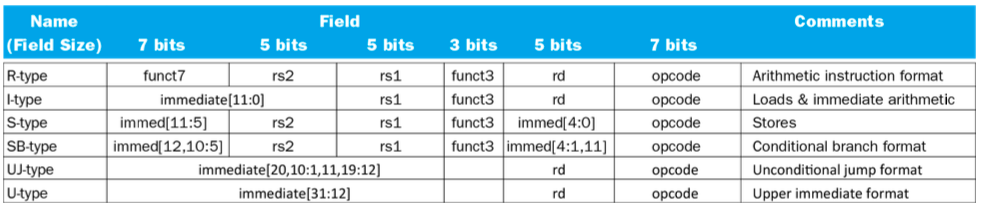
\includegraphics[width=\textwidth]{./images/rvencodings}
\caption{RISC-V ISA Encoding Formats \cite{lecture04riscv}.}
\label{fig:rve} % \ref{fig:rve}
\end{figure} 
From Figure \ref{fig:rve}, it is possible to see that the opcode, the source operands (\texttt{rs1} and \texttt{rs2}) and destination operand (\texttt{rd}) are maintained in the same bit positioning in order to reduce the decoding phase complexity.
The integer register file, used by all integer instructions, is composed of 32 general-purpose 32-bit registers.
\begin{table}
\centering
\begin{tabular}{| p{1.5cm} | p{1cm} | p{3.5cm} | p{2cm} |}
    \hline
    \textbf{Register} & \textbf{ABI Name} & \textbf{Description} & \textbf{ABI Saver}\\ \hline
    \texttt{x0} & \texttt{zero} & Hard-wired zero & / \\ \hline
    \texttt{x1} & \texttt{ra} & Return address & Caller \\ \hline
    \texttt{x2} & \texttt{sp} & Stack pointer & Callee \\ \hline
    \texttt{x3} & \texttt{gp} & Global pointer & / \\ \hline
    \texttt{x4} & \texttt{tp} & Thread pointer & / \\ \hline
    \texttt{x5} & \texttt{t0} & Temporary/alternate link register & Caller \\ \hline
    \texttt{x6-7} & \texttt{t1-2} & Temporaries & Caller \\ \hline
    \texttt{x8} & \texttt{s0/fp} & Saved register/frame pointer & Callee \\ \hline
    \texttt{x9} & \texttt{s1} & Saved register & Callee \\ \hline
    \texttt{x10-11} & \texttt{a0-1} & Function arguments/return values & Caller \\ \hline
    \texttt{x12-17} & \texttt{a2-7} & Function arguments & Caller \\ \hline
    \texttt{x18-27} & \texttt{s2-11} & Saved registers & Callee \\ \hline
    \texttt{x28-31} & \texttt{t3-6} & Temporaries & Caller \\ \hline
    \hline
\end{tabular}
\caption{RISC-V Integer Register File summary.}
\label{tab:iregfile} % \ref{tab:iregfile}
\end{table}
Table \ref{tab:iregfile} shows the registers names together with the ABI conventions. Notice that the program counter is not part of the register file itself, as the software cannot directly address it.\vspace{5mm} \newline
Part of the implemented ISA is also the Integer Multiplication and Division extension \textbf{RV32M}, which contains instructions that multiply or divide values held in two integer registers (see Table \ref{tab:iregfile}). The reason that made designers to separate multiply and divide out from the base integer is because usually multiplications and divisions operations are either infrequent or better handled by specialized accelerators. Thanks to this extension, the ISA can support multiplications, divisions, and reminder operations (No operation allows computing both Quotient and Reminder of a division).\vspace{5mm} \newline
The last extension implemented is the Control and Status Registers extension \textbf{Zicsr}, containing instructions needed to operate on CSRs registers. CSRs are a particular class of registers that can only be addressed by the Zicsr instructions and they are primarily used by privileged architecture to perform very specific tasks, e.g., handling exceptions, interrupts and traps. RISC-V ISA counts a total amount of 4096 CSRs but allow to implement just a subset of them. Our platform, for example, includes only those required for handling exceptions, interrupts, traps and for supporting User and Machine privilege levels.

\subsection{Privilege Levels}
Privilege levels are used to provide a protection mechanism, embedded in the hardware itself, between the different components of software stack, in such a way that any attempt to perform operations not permitted by the current privilege mode will rise an exception.
\begin{figure}[h!]
\centering
\vspace{0.5cm}
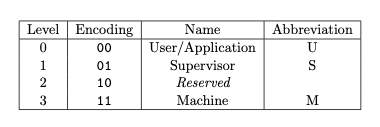
\includegraphics[scale=0.9]{./images/rvprivileges}
\caption{RISC-V Supported Privileges \cite{riscvII}.}
\label{fig:rvpri} % \ref{fig:rvpri}
\end{figure}
Figure \ref{fig:rvpri} shows all privilege modes supported by a RISC-V machine. These modes are listed in order of increasing privilege, where \emph{Machine} mode is the most privileged and \emph{User} mode being the least. All RISC-V systems must implement the \emph{M} mode, while the other are optional extensions.\\Thus, any RISC-V platform must fall in one of the following configurations, depending on the requirements:
\begin{itemize}
\item \textbf{M} \\ Simple embedded system.
\item \textbf{M, U} \\ Secure embedded system.
\item \textbf{M, S, U} \\ Systems running Unix-like operating systems.
\end{itemize}
When designing a RISC-V platform, the proper set of privileges must be carefully chosen based on the complexity of the software it will run. For instance, a small device that runs a single, \emph{thrusted} application may choose to only support \emph{Machine} mode: in this case, the application must be secure because it has full low-level access to the hardware. The modality \emph{Machine - User} is suitable for secure embedded systems. It provides a level of isolation between the application and a direct access to the hardware, by using \texttt{ecall} instruction to perform machine-level operations, that can fully and directly access the hardware. The full software stack separation is reached when the machine implements the \emph{Machine - Supervisor - User} mode. In this case the ISA is able to support a more robust system where there is an operating system working as intermediate between user and hardware.\vspace{5mm} \newline
Since our microcontroller is intended to be used as a security platform, it implements both \emph{M} and \emph{U} privileges required for a secure embedded system.
\begin{figure}[h!]
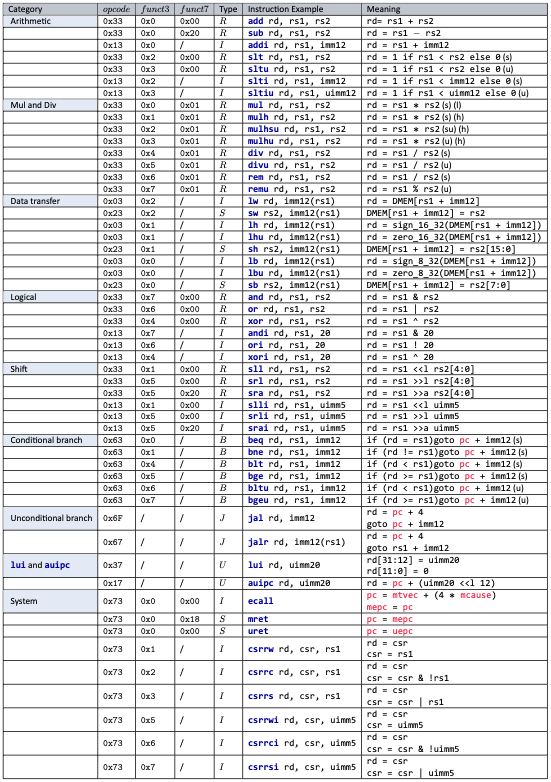
\includegraphics[scale=0.7]{./images/mc2101isa}
\caption{Implemented Instruction Set \cite{aftabManual}.}
\label{fig:mc2101i} % \ref{fig:mc2101i}
\end{figure}

\section{RISC-V Importance in IoT era}
Provided the main features of the RISC-V ISA, it should be clear the advantage that a modular architecture of this type can bring in terms of design freedom and use cases. In fact, the various extensions allow to design any kind of chip, from very small 16-bit low-power and cost-constrained microcontrollers, to extremely complex 64-bit full-featured high-performance SoCs. But why is there any need for a new instruction set architecture when there are several popular commercial ISAs available, that could be reused avoiding the significant effort and cost of porting software to a newer one?

The first reason behind the adoption of the RISC-V ISA as the standard architecture in academia and research is that all popular commercial ISAs, like x86 or ARM, are \emph{proprietary}. This means that vendors have a lucrative business in selling implementations, both in form of IP cores and silicon. Because of this, it is economically not sustainable for many companies, universities, or individuals, to develop custom designs. Another reason is that all popular commercial ISAs are massively \emph{complex}. In particular, the increasing complexity of legacy microprocessors has become profound, requiring hundreds of engineers, millions in investment, years in development, and all this complexity lead to a very inefficient and power-hungry design, for sure not suitable for IoT applications. It is therefore very difficult to fully implement one of those legacy architectures. Also, there is a little incentive to create subset ISAs, for more specialized design, because the software cannot run without being modified as well. For the aforementioned reasons, having an open source architecture like RISC-V, with tons of materials available for free, as well as a wide variety of projects going on, is a fundamental architecture that can help to overcome the barriers imposed by proprietary solutions. Among all the available open-source RISC-based ISA, RISC-V was designed to face these problems, through its modular architecture that allows to be used in any kind of applications, suitable also for educational purposes thanks to the simple base integer subset.

\begin{table}
\centering
\begin{tabular}{| p{4cm} | p{4cm} | p{4cm} | p{4cm} |}
 \hline
 \textbf{Barriers} & \textbf{Legacy ISA} & \textbf{RISC-V ISA}\\ \hline
 \hline\hline
 Complexity & 1500+ instructions, incremental ISA & 47 base instructions, modular ISA \\ 
 \hline
 Design freedom & \$\$\$ - Limited & Free - Unlimited  \\
 \hline
 License and Royalty fees & \$\$\$  & Open Source  \\
 \hline
 Design ecosystem & Moderate & Growing rapidly. Numerous extensions, numerous open cores. \\
 \hline
 Software ecosystem & Extensive & Growing rapidly \\
 \hline
\end{tabular}
\caption{Summary of RISC-V advantages with respect to Legacy ISAs \cite{riscvIntro}.}
\label{tab:legacy} % \ref{tab:legacy}
\end{table} 

The Table \ref{tab:legacy} is useful to summarize the advantages that the RISC-V ISA can offer with respect to popular commercial ISAs. These are the main reasons that allowed RISC-V to grow and become the today standard ISA used for embedded systems design in academia and research world.

It is important to underline that RISC-V is not only a revolution for hardware design in academia and research: it is also cracking a new commercial market wide open. As the IoT era keeps growing day by day, more and more companies are starting to develop their own chip, and companies that long prized for their proprietary architectures, like ARM, Intel and others, suddenly have to contend and compete with this new way of thinking and building. Therefore, it is essential that universities train engineers capable of designing efficient and reliable microarchitectures and also that the research can continue to produce innovative ideas that allow IoT technology to be widespread.

\section{State of the Art in Embedded System Design}
In this Chapter, some relevant state-of-the-art works are presented, featuring relevant scientific works related to RISC-V. As the purpose of my thesis is the design of a microcontroller, this Chapter discusses some of the most popular open-source RISC-V based SoCs, designed for energy-efficient computing. To stress again on the wide possibility that the RISC-V ISA can offer, three different types of architecture are here presented. 

The first one is the BOOM \cite{zhaosonicboom} SoC, part of the Berkeley Hardware CPUs, a very complex platform with an infrastructure usable for personal, supercomputer and warehouse-scale computers. The second example is about PicoRV32 \cite{picorv32} by Claire Wolf, a 32-bit microcontroller class RV32IMC implemented in Verilog HDL. The third and last example focuses on PULPino \cite{pulpino} from ETH Zürich and University of Bologna, which is a simple microcontroller that can be extended for being used as custom embedded DSP. The architecture of this last microcontroller has been particularly important for my thesis work, because it has been used as a reference.

\subsection{Berkeley Out of Order Machine}
The BOOM machine is a synthesizable and parameterizable open-source RV64GC RISC-V core, written in Chisel \cite{chisel}. As its name suggest, BOOM is an out-of-order processor, inspired by the MIPS R10000 \cite{491460} and the Alpha 21264 \cite{755465} processors . Created at the University of Berkeley (California) in the Berkeley Architecture Research group, its focus is to provide a high performance, synthesizable and parameterizable SoC for architecture research. This is a perfect example to underline how much degree of complexity can be reached by using RISC-V extensions.

\begin{figure}[h!]
\centering
\vspace{0.5cm}
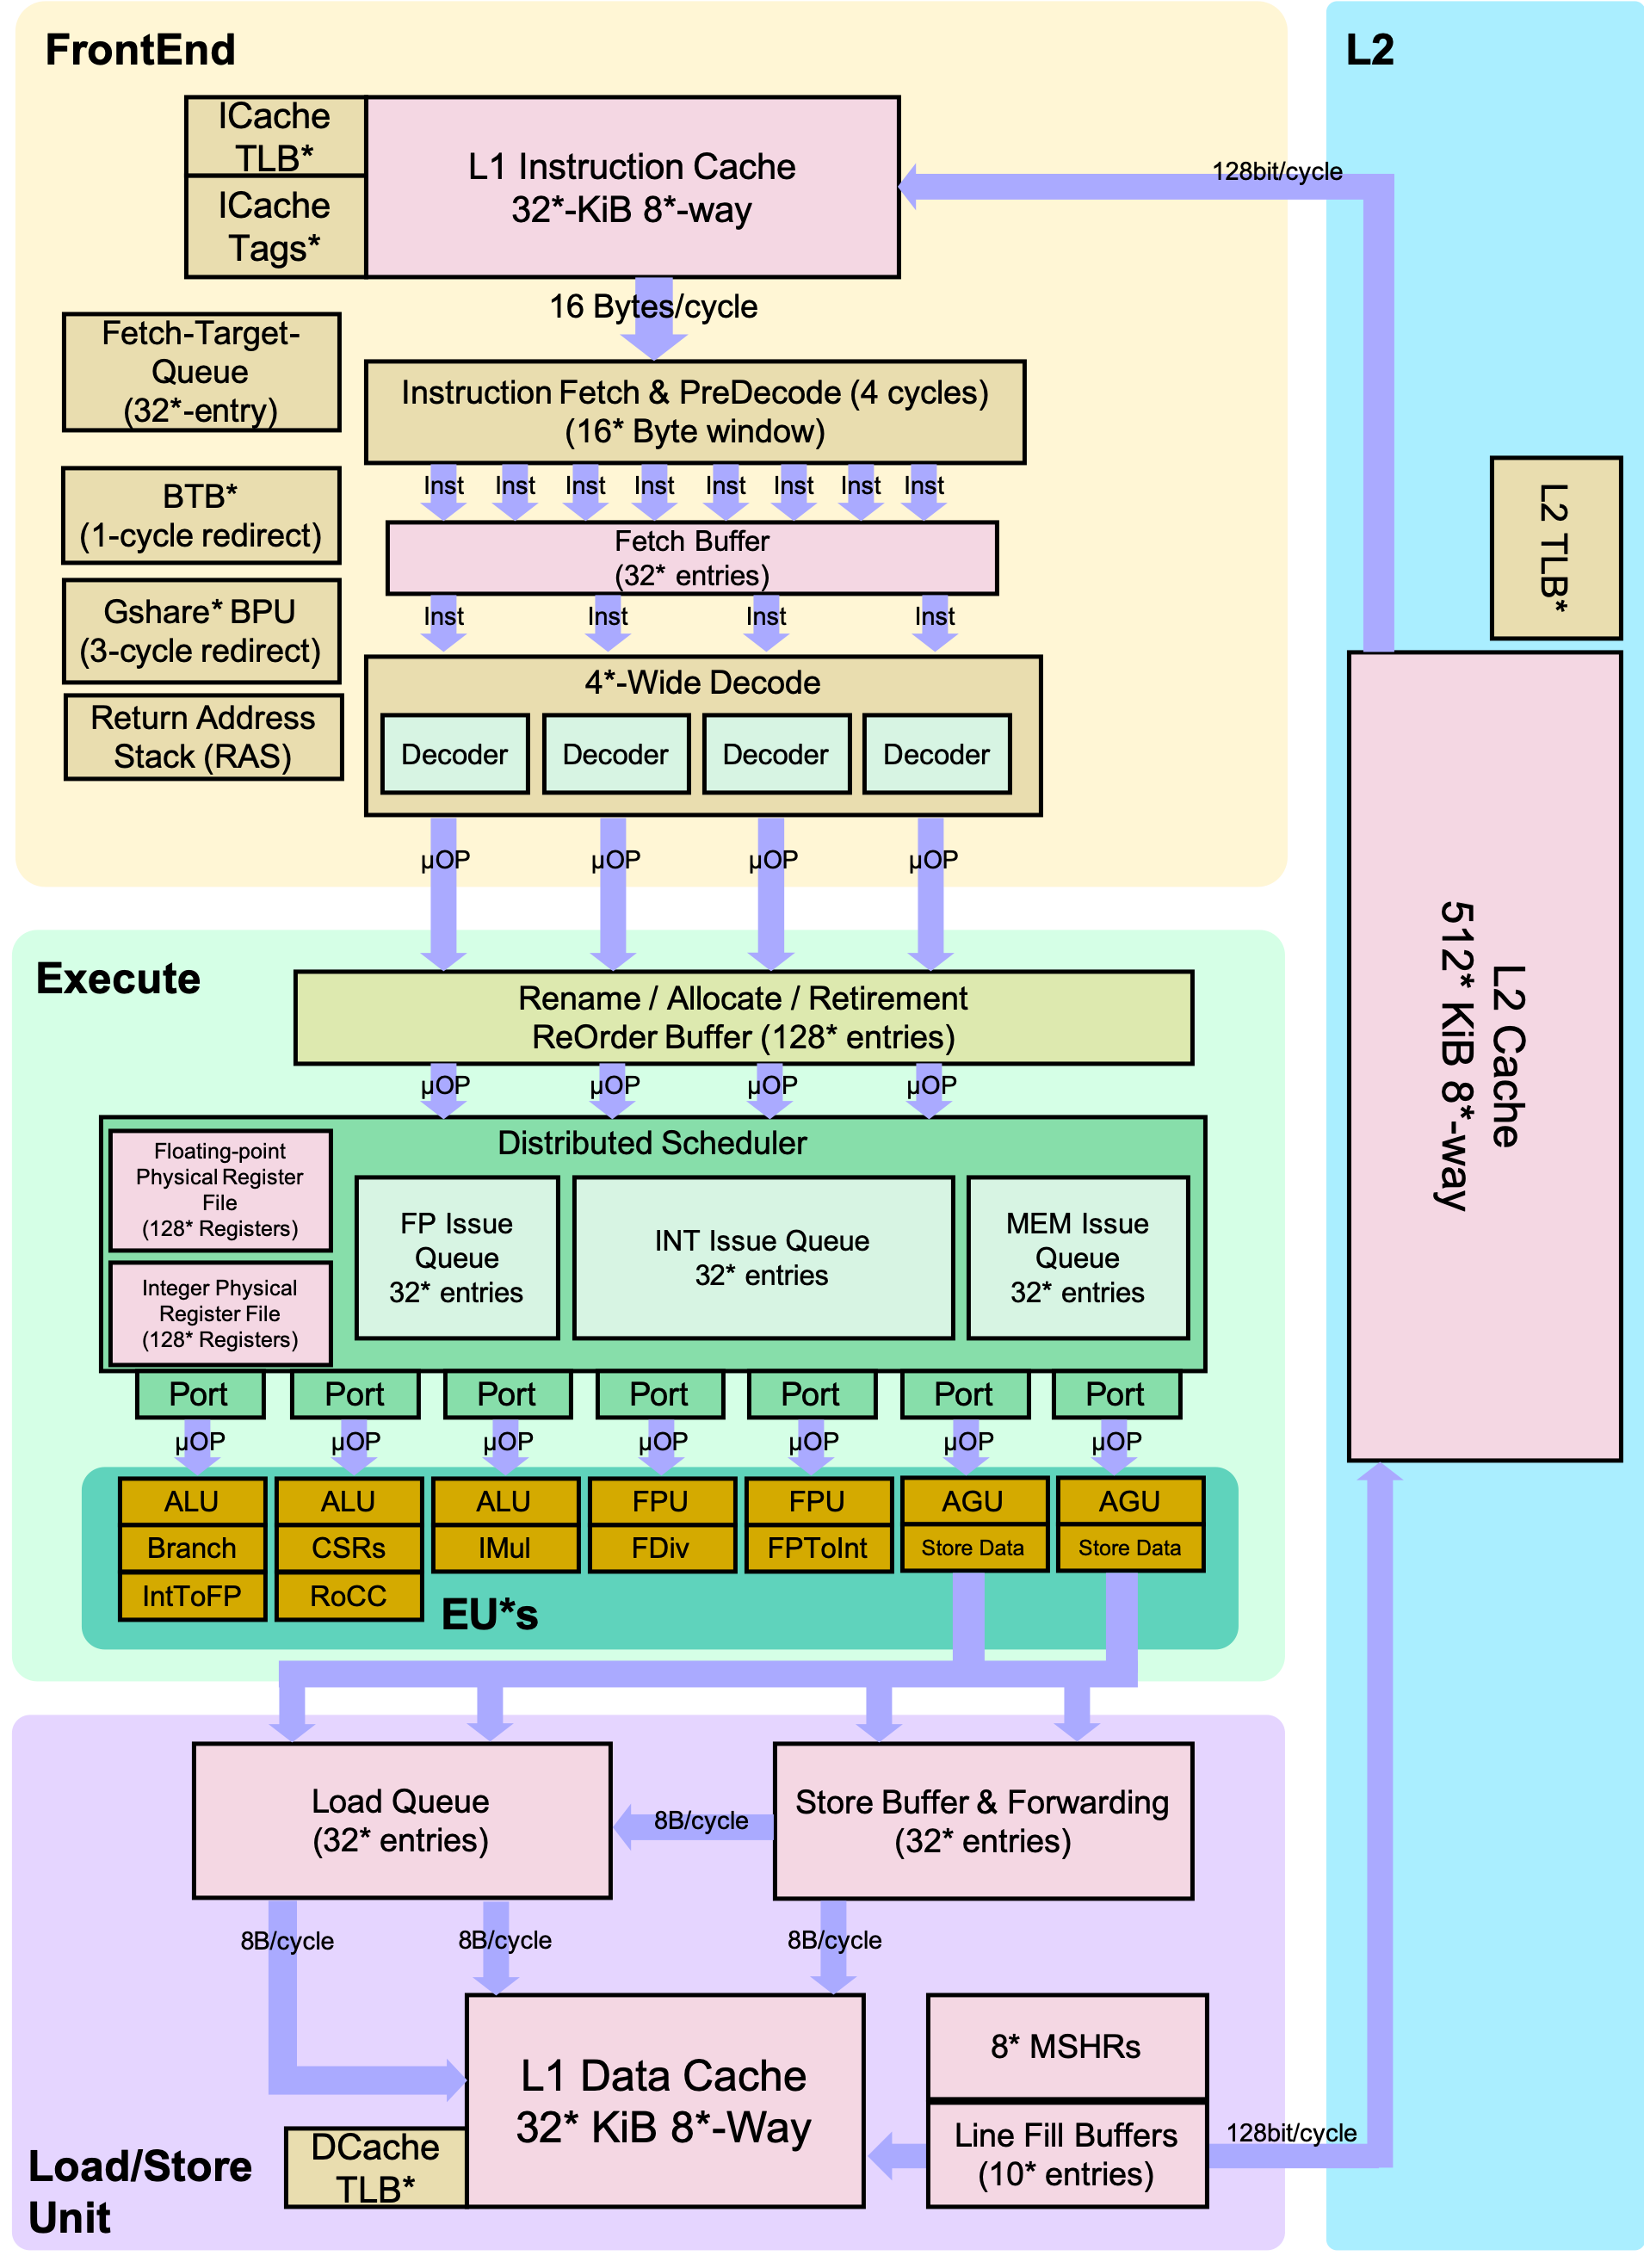
\includegraphics[scale=0.2]{./images/boom-core}
\caption{BOOM Architecture Overview \cite{zhaosonicboom}.}
\label{fig:boom} % \ref{fig:boom}
\end{figure}

From Figure \ref{fig:boom}, it is possible to distinguish the classical pipeline stages of out-of-order architectures. Conceptually, the processor implements 10 stages: \texttt{Fetch}, \texttt{Decode}, \texttt{Register Rename}, \texttt{Dispatch}, \texttt{Issue}, \texttt{Register Read}, \texttt{Execute}, \texttt{Memory}, \texttt{Writeback} and \texttt{Commit}. The architecture is then able to execute instructions in out-of-order fashion, pushing even more the throughput and performances of a standard pipeline. The fact that it also implements a 64-bit version of the standard \texttt{G} indicates this core is designed exclusively for high performance systems.

Further details can be found in the official Github repository\footnote{\url{https://github.com/riscv-boom/riscv-boom}}, where it is also possible to access at the RTL description.

\subsection{Picorv32 microcontroller}
The PicoRV32 is a microcontroller that implements the RV32IMC instruction set written in Verilog. This microcontroller can be configured in many different ways, starting from the core itself that can be configured to support the following extensions: \texttt{RV32I}, \texttt{RV32IC}, \texttt{RV32IM} and the \texttt{RV32IMC}. The architecture of the microcontroller is also available in the following configurations:

\begin{itemize}
\item \texttt{picorv32}: simplest version that implements a simple native memory interface, usable in simple environments;
\item \texttt{picorv32\_axi}: provides an AXI-4 Lite Master interface that can be easily integrated within other systems based on AXI standard bus infrastructure;
\item \texttt{picorv32\_wb}: provides a Wishbone bus master interface;
\item \texttt{picorv32\_axi\_adapter}: This core provides a bridge between the native memory interface and an AXI4 infrastructure. This implementation can be used to create custom cores that include one or more \texttt{picorv32} cores together within a compact microcontroller that internally can communicate using a native custom lightweight interface, and externally can be attached through AXI4.
\end{itemize}

It is possible to understand that this embedded system is meant to be used as auxiliary processing device in FPGA designs and ASICs. The architecture includes also a UART peripheral and a SPI Flash Controller.
Any additional information can be found in the official Github repository\footnote{\url{https://github.com/YosysHQ/picorv32}}.

\subsection{PULPino}
Developed by ETH Zurich and the University of Bologna, PULPino is a RISC-V-based single-core SoC written in SystemVerilog, which represents a small part (one core) of the Parallel Ultra-Low Power (PULP) platform designed for energy-efficient IoT parallel computing.

In Particular, the PULP SoC is a cluster that embeds a configurable number of RISC-V based cores with a design focused for being extremely low power consuming. Perfectly suited for IoT devices that requires high computational capabilities. PULPino represents a first step towards the release of the full PULP platform. In fact, PULPino inherits from its bigger brother some of the IPs and the core, focusing on ease of use and simplicity.

\begin{figure}[h!]
\centering
\vspace{0.5cm}
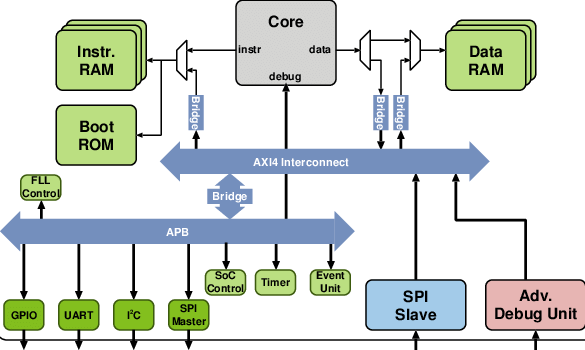
\includegraphics[scale=0.6]{./images/pulpino}
\caption{PULPino Microcontroller \cite{pulpino}.}
\label{fig:pulpino} % \ref{fig:pulpino}
\end{figure}

Figure \ref{fig:pulpino} shows the design overview of the SoC. From an architectural point of view, it is a simple single-core AMBA-based embedded system. It offers a modular design that does not include complex features like caching mechanisms, memory hierarchy or DMA. The core is directly connected to the IRAM and DRAM in a single access, no waiting manner. There is a central AXI interconnection, that interconnects the processor with the memories, allowing pipelined high-bandwidth operations. Regarding the core, the microcontroller is based on a 32-bit RISC-V architectures and can be configured to use either the \texttt{RISCY} or the \texttt{zero-riscy} core. Both developed at ETH Zürich.

\begin{figure}[h!]
\centering
\vspace{0.5cm}
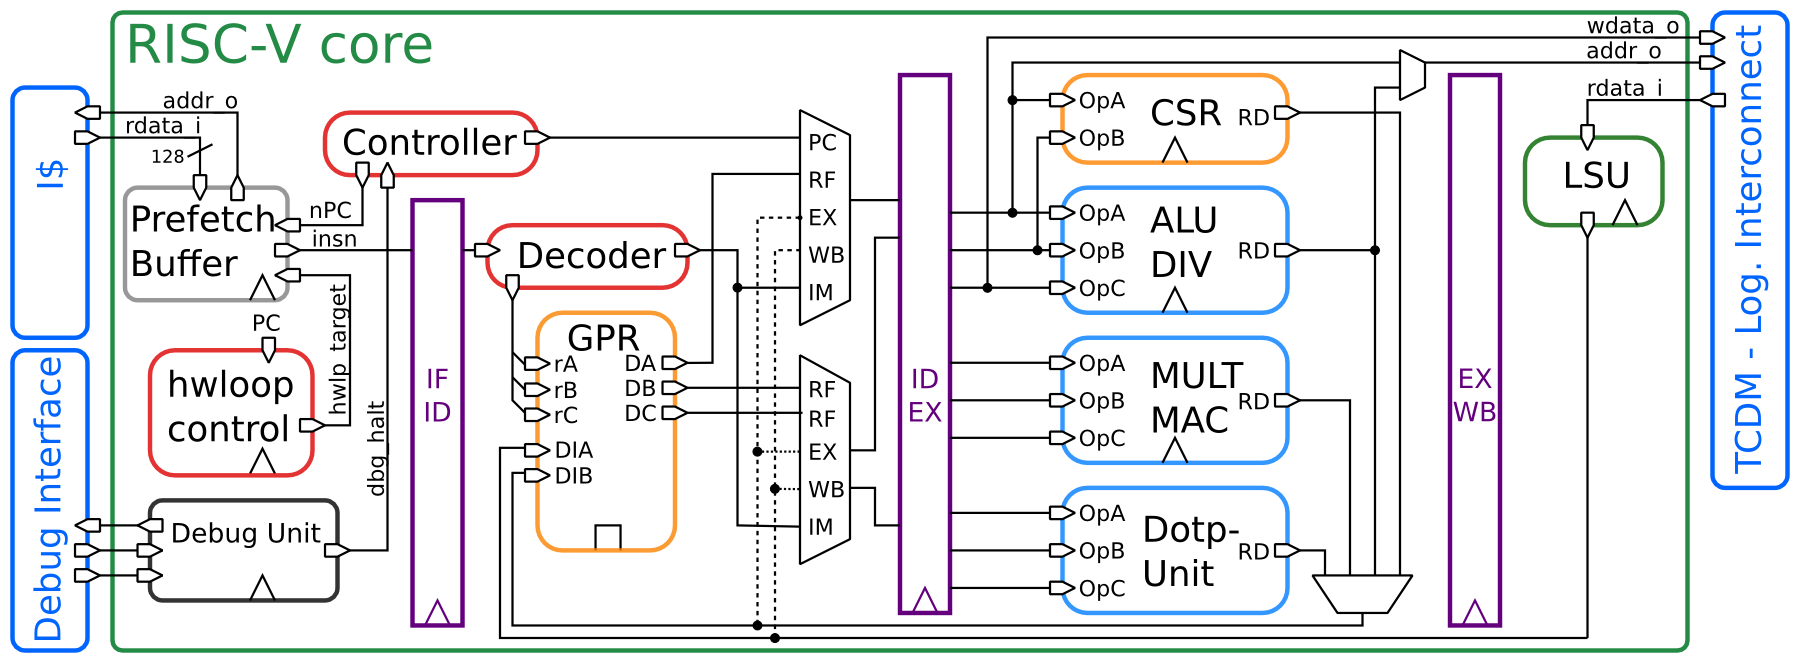
\includegraphics[scale=0.7]{./images/riscy}
\caption{RISCY core.}
\label{fig:riscy} % \ref{fig:riscy}
\end{figure}

The \texttt{RISCY} core, shown in Figure \ref{fig:riscy}, is an in-order, single-issue core with 4 pipeline stages able to guarantee an IPC close to 1. The ISA supports the base integer instruction set (RV32I), compressed instructions (RV32C), multiplication and division instruction extension (RV32M). In can also be configured to implement the RV32F extension for single-precision floating point operations. It also implements several custom ISA extensions such as hardware loops, post-incrementing load and store instructions, bit-manipulation instructions, MAC operations, fixed-point operations, packed-SIMD instructions and the dot product. All these additional features have been implemented for allowing ultra-low-power signal processing applications. Also, a subset of the 1.9 privileged instructions are supported.

\begin{figure}[h!]
\centering
\vspace{0.5cm}
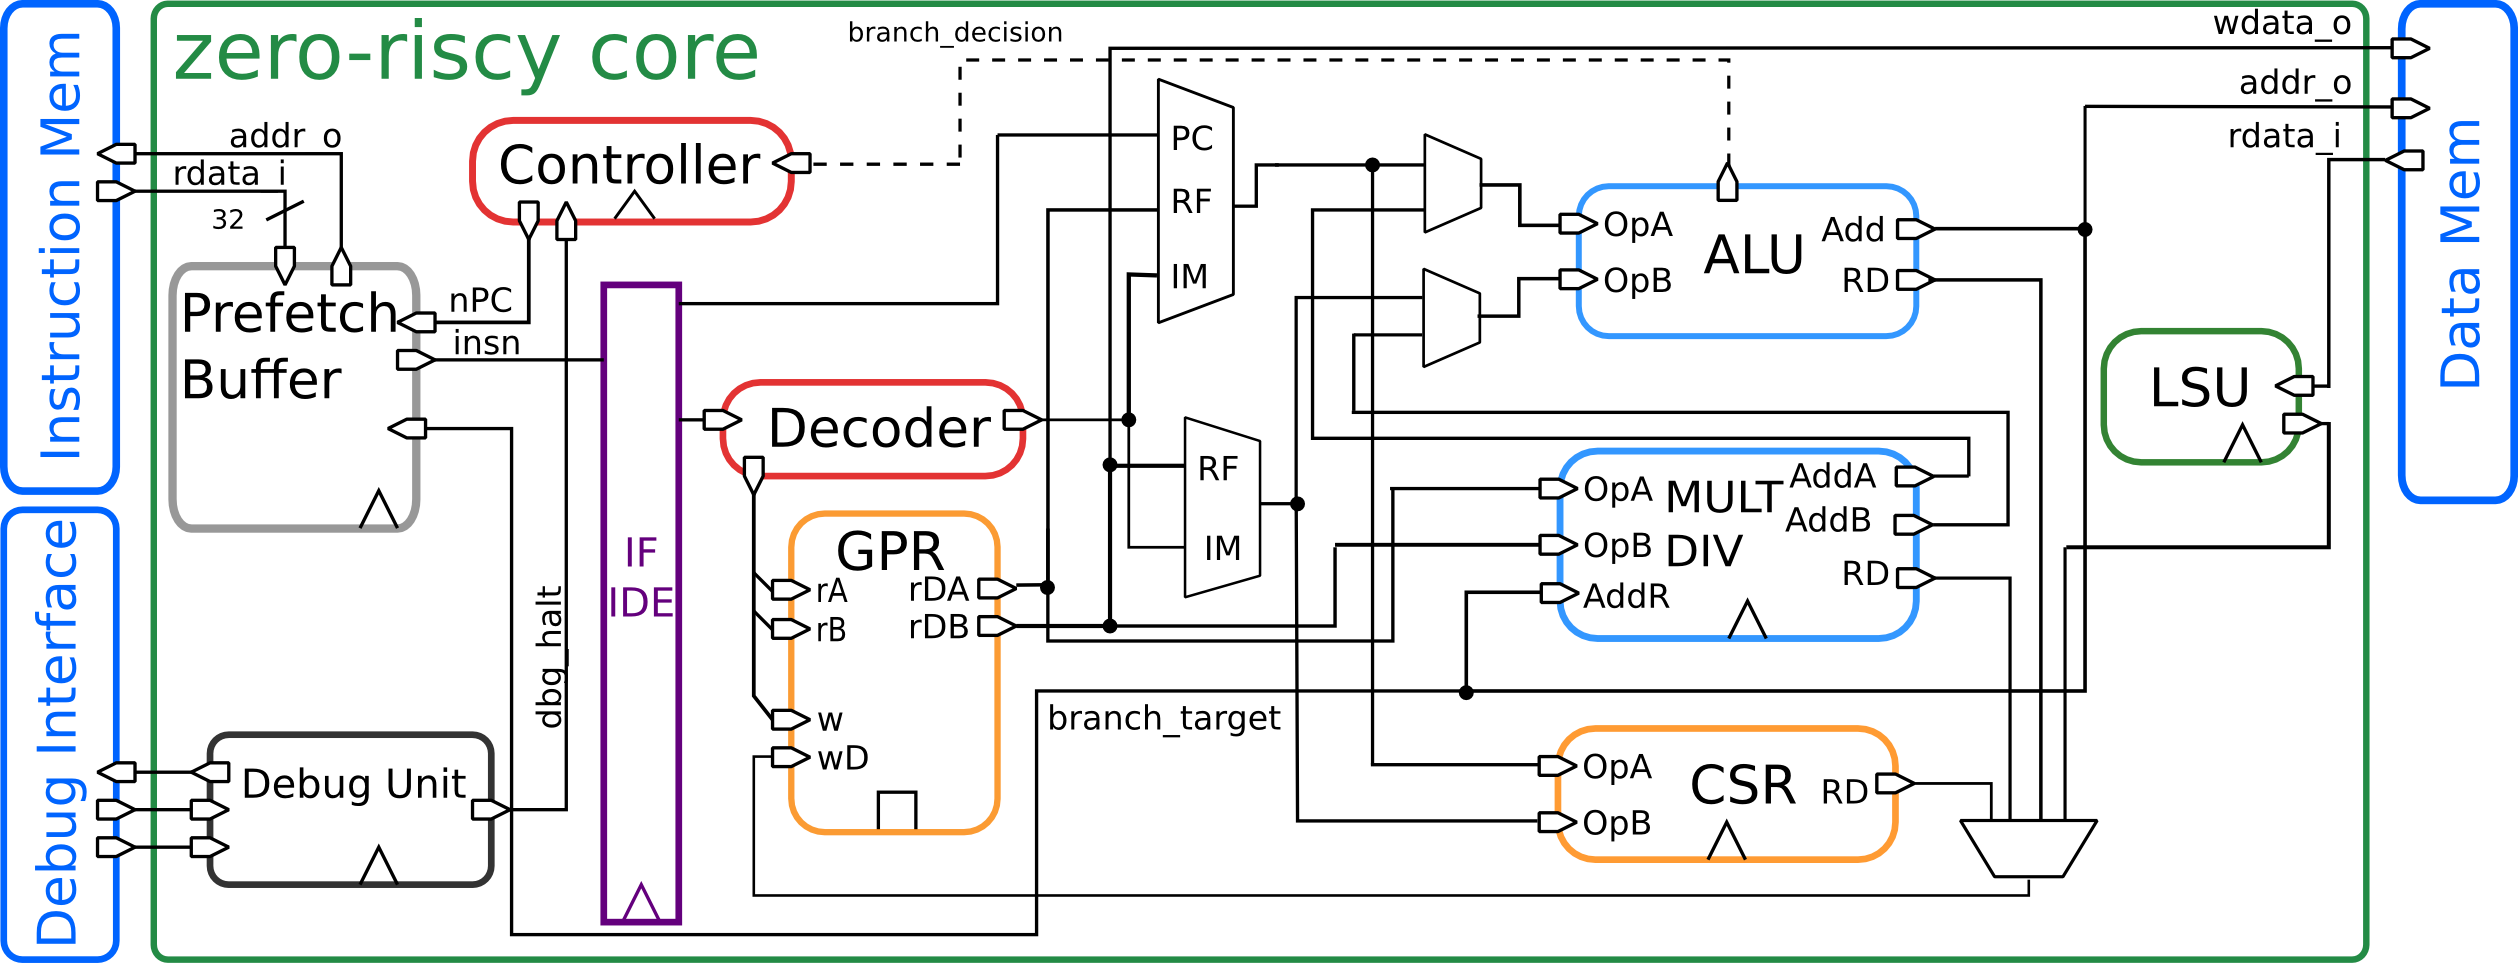
\includegraphics[scale=0.7]{./images/zeroriscy}
\caption{Zero-riscy core.}
\label{fig:zeroriscy} % \ref{fig:zeroriscy}
\end{figure}

The \texttt{Zero-riscy} core, depicted in Figure \ref{fig:zeroriscy}, is instead a much more simpler processor. Suitable for ultra-low-power ultra-low area constrained embedded systems. It is an in-order, single issue core with 2 pipeline stages supporting the RV32I, RV32C and a subset of 1.9 privileged ISA. Can also be configured to implement the RV32M and the reduced number of register extension RV32E. The architecture offers a secondary bus level that interconnects a broad set of peripherals for the communication with the outside world. Part of the implementations are also the SPI Slave and the Debug Unit, which are used to pre-load the RAMs with executable code from SPI flash and to allow access to the whole memory map via JTAG for debugging purposes.

Among all the available microarchitectures, PULPino is the one chosen to be our reference architecture. This is because it implements in a very simple and compact design all the features necessary to have a complete usable microcontroller-style platform, closer to our requirements. Also, what makes PULPino perfect for being used as a reference soft microcontroller is for sure its modular and clean design, the extensible software toolchain built around it for cross-compilation, RTL simulation and synthesis, together with a great documentation to support usage and learning.

The RTL description, as well as the entire toolchain for simulations, compilation and FPGA synthesis can be found in the official Github repository\footnote{\url{https://github.com/pulp-platform/pulpino}}.

\section{Our contribution to the RISC-V community}
Whenever an team of engineers decide to start designing a new RISC-V platform, the first possible way to act is to start from an already implemented open-source platform, like one of those seen before, where it is possible to include custom integrations and modify the existing design to fulfil the desired behaviour. The second choice would be to start a new design from scratch, by using some well known architecture as a reference. There are two factors on which the choice of the path to take is based: the first one regards the specifications and use cases of the embedded device. For instance, if the target is to design a low-power IoT device, if one wants to start from something already developed, he or she must have a soft lightweight microcontroller to customise, otherwise there is the need to start a new design from scratch. The second factor is related to the technical background of the team on HDL languages, which require a certain degree on know-how in order to develop clean and synthesizable designs. Embedded Systems engineers in Politecnico di Torino, for example, have strong expertise in VHDL, but not in SystemVerilog or Chisel HDLs, and this reflects to the students.

Regarding our RISC-V based platform MC2101, the research team that hosted me needed to have a RISC-V based architecture entirely customizable and synthesizable. The particular aim of our platform is to offer the possibility to integrate hardware security solutions and also to assess and evaluate them through software testing. Those kind of solutions first require a simple architecture that can be easily customised starting from the core itself, and then a proper toolchain for automating all the processes of RTL simulation, synthesis and compilation.

Among all the most popular solutions available in literature, the PULPino architecture mentioned before is for sure the one that comes closest to our needs. Referring again to the Figure \ref{fig:pulpino}, it is a modular design, easy to use, that includes all the set of peripherals necessary to interact with the microcontroller once synthesized on FPGA, as well as the necessary interfaces used to debug and flash the firmware on it. All these features are what is needed to test the architecture and any custom integration. Of great importance is also the \emph{software toolchain}, created with the aim of automating all the processes of synthesis, RTL simulations, and software compilation. The big problems with PULPino, common to many other RISC-V most popular open-hardwares, is that it is fully described using SystemVerilog hardware description language, which is not part of our background as computer engineers.

It was therefore mandatory to opt for our own design, developed from scratch, fully implemented in VHDL. The AFTAB processor, briefly described in the next Section, was the first step of the development.

\section{The AFTAB Processor}
AFTAB, acronym for ``A Fine Turin/Tehran Architectural Being'', is an in-order fully sequential (not pipelined) 32-bit RISC-V core, developed by the CINI Cybersecurity National Laboratory in cooperation with University of Tehran. The processor works according to the Von Neumann architecture, so there is only a single RAM containing both data and instructions.

As for the implementation details, its enough to give a high-level description of the processor, starting from its interface and going directly to the programmer's model.
\subsection{AFTAB Interfacing Ports}

\begin{figure}[h!]
\vspace{0.5cm}
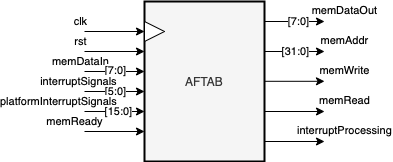
\includegraphics[scale=0.9]{./images/aftabpins}
\caption{AFTAB microprocessor interface.}
\label{fig:aftabpin} % \ref{fig:aftabpin}
\end{figure}

The core can be described as a blackbox component (Figure \ref{fig:aftabpin}), whose pins can be grouped into the Memory Interface set and the Interrupt Interface set. The Memory Interface includes these signals:

\begin{itemize}
\item \texttt{memRead} \& \texttt{memWrite}: read and write signals for the memory. Forwarded in the MC2101 bus in order to start a transaction that can target the main memory or any peripheral
\item \texttt{memReady}: fundamental signal used to stall the processor in the fetch stage. In this way, by controlling this signal, the bus infrastructure can take the necessary time to complete read and write operations;
\item \texttt{memAddr}: AFTAB address bus is 32-bit wide;
\item \texttt{memDataIn} \& \texttt{memDataOut}: two 8-bit ports that together build the data bus of the microcontroller. During load and store operations, they carry variable number of bytes per transaction (1, 2, or 4) in a sequential way, so that only one byte per clock cycle can be read or written.
\end{itemize}

As for the Interrupt Interface set, there are a total of 22 independent interrupt lines, where 16 of them are for platform use, plus an additional signal (\texttt{interruptProcessing}) indicating when the processor is in the interrupt processing states. The core is also able to handle the following hardware-level exceptions:

\begin{itemize}
\item \textbf{Illegal Instruction}: the decode phase does not recognise the opcode as a valid one;
\item \textbf{Illegal CSR instruction}: raised when there is an attempt to read or write a CSR register with an inappropriate privilege level, or when trying to access a non-existing CSR register;
\item \textbf{Instruction address misaligned}: raised after an attempt to access the instruction memory without the proper 4-bytes alignment.
\end{itemize}

For the programmer's point of view, as previously anticipated, AFTAB implements the RV32I, RV32M, and Zicsr extensions. Therefore, the instruction set supported is the one depicted in Figure \ref{fig:mc2101i}, and the registers available are the integer ones, listed in Figure \ref{tab:iregfile}.

The RTL description, as well as the entire toolchain for simulations, compilation and the manuals can be found in the official Github repository\footnote{\url{https://github.com/RHESGroup/aftab}}.
%\input{chapters/related_work.tex}
\chapter{Design and Development of MC2101}
The present Chapter is entirely dedicated to MC2101 microcontroller. The first Section explains the hardware-level architecture of MC2101, from the bus infrastructure to the various peripherals, and all the related design and development choices. The software part is described in the second Section, dedicated precisely to describe all the implemented system's libraries provided to support the programmer job with a proper set of low-level C functions, useful to program all peripherals without the need of accessing their registers ``by hand''. A third Section is dedicated to the testing part, in particular to the testing methodology followed to assess the functional correctness of the various designed hardware components, and their interconnection. The same Section is also dedicated to describe how does the serial communication between FPGA and a PC have been implemented, with the purpose of providing a way to allow the interaction between a personal computer and the synthesized MC2101, through a command-line terminal.

\section{MC2101 architecture}
MC2101 microcontroller has been designed with the purpose of being used as a synthesizable and extensible platform for integration and assessment of security solution for IoT implemented inside the AFTAB processor. At the current state, the microcontroller is composed of a minimal set of peripherals properly selected for providing all necessary input/output functionalities useful for interacting with the external world, once synthesized on a FPGA.

%\begin{figure}[h!]
\begin{figure}[h]
\vspace{0.5cm}
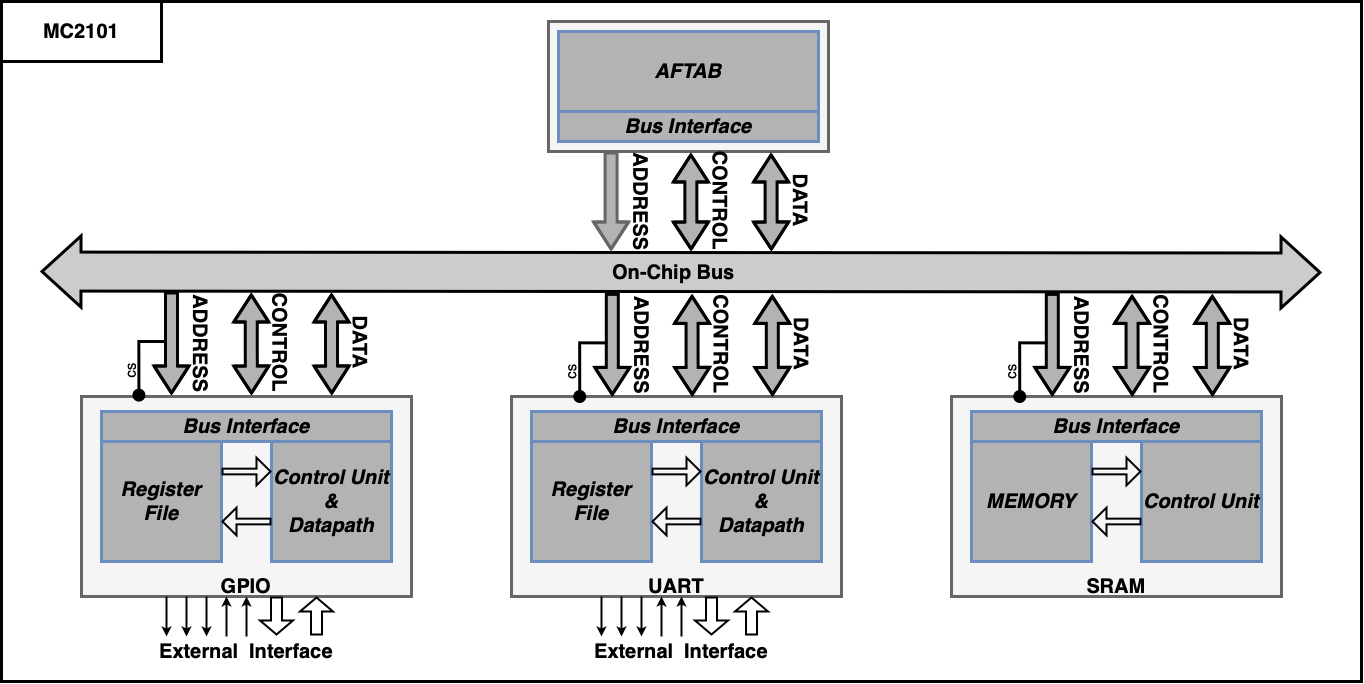
\includegraphics[width=\textwidth]{./images/MC2101}
\caption{MC2101 microcontroller.}
\label{fig:mc2101} % \ref{fig:mc2101}
\end{figure}

The Figure \ref{fig:mc2101}  shows the design overview of the microcontroller. The architecture includes a single bus, which provides the system with the proper hardware infrastructure necessary to interconnect the AFTAB processor with all peripherals and the main memory. The processor plays the role of the master: it is the only component able to initiate transactions on the bus, which can be composed of single or multi-cycles read/write operations. Peripherals and main memory are accessed by AFTAB using the memory-mapped mode: this means that the entire address space includes both peripherals and main memory. Therefore, the processor uses the same load/store instruction for accessing all components attached to the bus.

The communication between the processor and any peripheral happen only through the peripheral's register file, which can contain three different type of registers, with different read/write policy:

\begin{itemize}
\item \textbf{Control Registers}: used to configure the peripheral functionalities. They are written by the processor and read by the peripheral;
\item \textbf{Status Registers}: used to report the current state of the peripheral. Written by the peripheral and read by the processor;
\item \textbf{Data Registers}: used to exchange data. Both processor and peripheral can read and write on them.
\end{itemize}

The size and the number of registers depends on the functionalities implemented by the peripheral, which can be for instance a 32-bit peripheral, with 32-bit register file or a 8-bit peripheral with 8-bit registers. 

The bus implements three different types of interconnections:

\begin{itemize}
\item \textbf{Data Lines}: set of independent read and write data signals used to read and write data on peripherals registers and on the main memory;
\item \textbf{Control Lines}: used to provide signals for controlling read or write operations and for allowing peripherals and main memory to feedback the processor about the current state of the transaction;
\item \textbf{Address Lines \& Chip Select}: the most significant bits of the address lines pass through a decoder that drives all chip select signals: in this way, the peripheral is activated only when necessary.
\end{itemize}

Each component attached to the bus must include the Bus Interface, which is a sort of wrapper to be placed around each component in such a way to bridge signals coming from the bus to the internal hardware (FSM + Datapath) of the peripheral and vice versa. Peripherals can implement an additional External Interface, which is used to handle the communication to the external world. In particular, the conversion of incoming external asynchronous digital signals into the synchronous domain of the microcontroller.

In the following Subsection, some more details of the microcontroller design are reported, in order to present what are the functionalities supported by the system and the relative design choices made.

\subsection{Bus Infrastructure}
In the microcontroller development, the bus infrastructure was the first item to be addressed because of its vital role in interconnecting the whole system. In literature, there exist a lot of bus architectures which, over the years, have evolved to become an open-standard in SoCs design. In particular, the the most used open-source architecture is the ARM AMBA bus \cite{ambaAHB} \cite{ambaAPB}, that, thanks to its modular design engineered to support high-performance and low power on-chip communications, is today a standard \emph{de facto}, used in most of the SoCs present on the market. The problem with such solutions is that they implements sophisticated features, designed to be used in full-featured high-performance microcontrollers much more complex than our embedded system. In particular, the absence of a pipeline in the our processor prevents the usage of AMBA solutions, that are in fact designed to pipeline all the communications in order to increase the throughput.

The idea was to take inspiration from a standard architecture (AMBA and Avalon, for instance) to build a simpler infrastructure. In particular, the designed architecture preserves a minimal subset of AMBA specifications to build a simpler infrastructure, suitable for our needs, that remains modular and upgradable at the same time.

\begin{figure}[h]
\vspace{0.5cm}
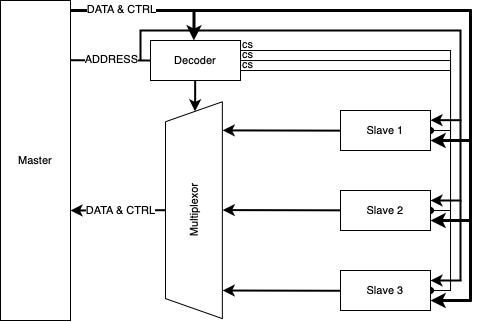
\includegraphics[scale=0.8]{./images/BUS}
\caption{MC2101 Bus Block Diagram.}
\label{fig:bus} % \ref{fig:bus}
\end{figure}

Figure \ref{fig:bus} shows the block diagram of the bus system. It is an infrastructure that supports a single master with multiple slaves, thus no arbitration mechanism has been implemented. The bus interconnection logic consists of a single centralised address decoder and a slave-to-master multiplexor. The decoder monitors the address lines driven by the master so that the appropriate slave is selected during each transaction. It also provides control to the multiplexor, which is in charge of routing the corresponding slave output back to the master.

%\begin{figure}[h!]
\begin{figure}[h]
\vspace{0.5cm}
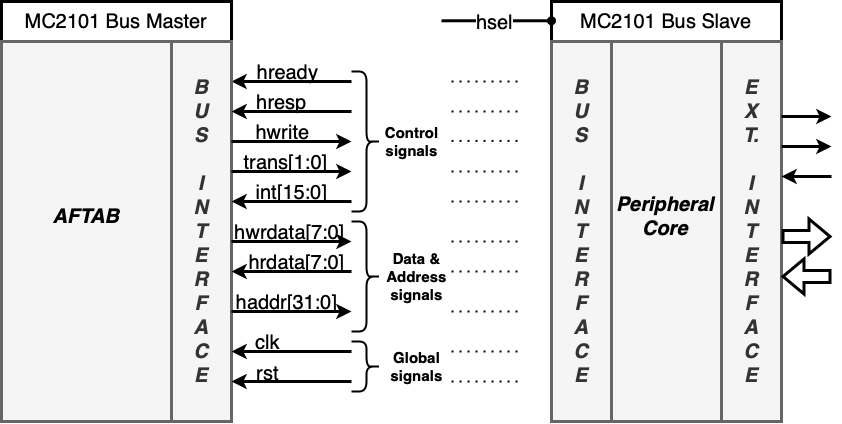
\includegraphics[scale=0.5]{./images/MasterSlave}
\caption{Master \& Slave Interfaces.}
\label{fig:masterslave} % \ref{fig:masterslave}
\end{figure}

The bus master interface, on the left of Figure \ref{fig:masterslave}, provides address and control information to initiate read and write operations.
The slave, whose interface is shown on the right of Figure \ref{fig:masterslave}, responds to transfers initiated by the master, by using a \texttt{hsel} (chip select) signal from the decoder to control when to respond a request. When selected, the slave will start monitoring the bus lines in order to respond to commands from the master. Therefore, all the slaves will stay into an idle state until they are individually waken up by a signal.\vspace{5mm} \newline 
Each slave is also able to feedback the master about:
\begin{itemize}
\item the success
\item the failure
\item or the waiting of the data transfer
\end{itemize}
by using the \texttt{hresp} and \texttt{hready} dedicated lines. In this way, a slave is able to extend the data phase when extra time is needed, but also to inform the rest of the system that some bad operations are happening in the bus.
\begin{table}
\centering
\begin{tabular}{| l | l | p{7cm} |}
    \hline
    \textbf{Name} & \textbf{Type} & \textbf{Description}\\ \hline
    \texttt{hready} & Control & When driven LOW, the transfer is extended.  \\ \hline
    \texttt{hresp} & Control & When HIGH, indicates that the transfer status is on error.  \\ \hline
    \texttt{hwrite} & Control & Indicates the transfer direction. When HIGH the signal implies a write transfer, on the contrary when LOW a read transfer.\\ \hline
    \texttt{htrans[1:0]} & Control & Shows the current state of the bus.\\ \hline
    \texttt{int[15:0]} & Control & Independent interrupt lines, can be driven by peripherals to issue a IRQs. \\ \hline
    \texttt{hwrdata[7:0]} & Data & 8-bit data lines from the master to the slaves. \\ \hline
    \texttt{hrdata[7:0]} & Data & 8-bit data lines from the slave to the master.  \\ \hline
    \texttt{haddr[31:0]} & Address & Address space is on 32-bit, thus also the address line. \\ \hline
    \texttt{clk} & Global & global clock signal \\ \hline
    \texttt{rst} & Global & global reset signal \\ \hline
    \hline
\end{tabular}
\caption{Bus Signals.}
\label{tab:bussig} % \ref{tab:bussig}
\end{table}
The full list of signals is described in Table \ref{tab:bussig}.

In the following Subsections, the main features implemented in the GPIO and UART peripherals are presented. Together, they provide a set of minimal functionalities for interacting with the microcontroller from the external world.

\subsection{GPIO Peripheral}
The GPIO (General Purpose Input Output) is a peripheral module present in all embedded processors. It is used to manage sets of SoC's incoming and outgoing digital signals, by driving and checking the logic state of physical pins. GPIOs can be used in a diverse variety of applications, limited only by the electrical and timing specifications of the peripheral's interface, and the ability of software to interact with it in a sufficiently timely manner. In most of the cases, GPIOs are used to switch LEDs, interface the microcontroller to buttons, user-selectable switches or electronic switches (relays). In other cases, there is also the possibility to use GPIO as a bit banging communication interface, where software is used as substitute for dedicated hardware in order to implement a specific communication protocol, e.g., a software-based SPI bus with 4 GPIO pins.

\begin{figure}[h]
\vspace{0.5cm}
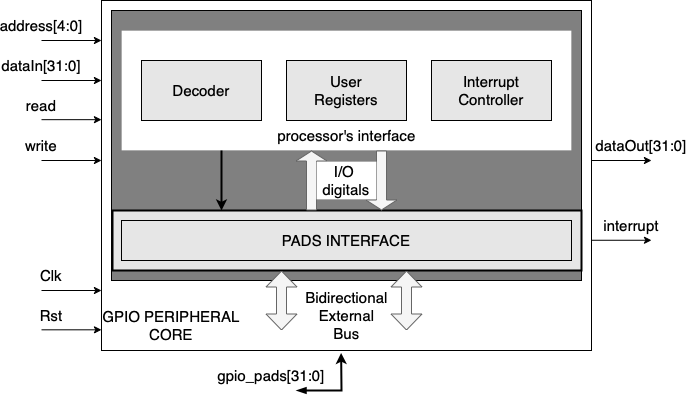
\includegraphics[width=\textwidth]{./images/GPIO}
\caption{MC2101 GPIO Peripheral Core.}
\label{fig:gpio} % \ref{fig:gpio}
\end{figure}

In Figure \ref{fig:gpio}, the core of the peripheral is showed, together with its relative set of signals coming from the Bus Interface and from the External Interface.
The GPIO is designed as a 32-bit peripheral, and so it provides a 32-bit processor's interface with 32-bit wide user registers and data bus (\texttt{dataIn} and \texttt{dataOut}). The conflict between MC2101's data bus, that is on 8-bit (see \texttt{hwrdata} and \texttt{hrdata} in Table \ref{tab:bussig}), and the peripheral's data bus are solved by the Bus Interface, which provides a bridge for the communications between the two domains. The External Interface (in Figure \ref{fig:gpio} as \emph{Pads Interface}) works as an intermediate between the bidirectional bus connected to physical pins and the peripheral's core. In particular, through the Pads Interface, the asynchronous bidirectional external lines (\texttt{gpio\_pads}) are separated into independent input and output lines, synchronised with the global clock.

The 5-bit \texttt{address} signal selects which user register is being access by the by the processor. As explained before, read and write operations on peripherals are enabled by a proper chip select signal. When the chip select condition is met, the Bus Interface rises one of the two strobe signals, \texttt{read} and \texttt{write}, for accessing the user registers. The GPIO provides also an \texttt{interrupt} line to the processor. This line will rise as soon as an interrupt condition occurs on any of the 32 pad lines. When this happen, the processor will have to execute appropriate read or write operations to deassert the interrupt. The peripheral, programmed through the user registers, is able to support the following functionalities:

\begin{itemize}
\item Control the input/output direction of each GPIO pads;
\item Enable interrupts for each input bits and configure the triggering behaviour on logic levels or rising/falling edges;
\item Drive and control external pins.
\end{itemize}

\begin{table}
\centering
\begin{tabular}{| p{2cm} | p{2cm} | p{2cm} | p{7cm} |}
    \hline
    \textbf{Name} & \textbf{Address} & \textbf{Access} & \textbf{Description}\\ \hline
    \texttt{PADDIR} & \texttt{0x1A100000} & R/W & Control the direction of each of the GPIO pads. A value of 1 means the pin is configured as output.  \\ \hline
    \texttt{PADIN} & \texttt{0x1A100004} & R & Saves the input values coming from input pins.\\ \hline
    \texttt{PADOUT} & \texttt{0x1A100008} & R/W & Drives the output lines with its content.\\ \hline
    \texttt{PADINTEN} & \texttt{0x1A10000C} & R/W & Interrupt enable bits for input lines.\\ \hline
    \texttt{INTTYPE} & \texttt{0x1A100010} & R/W & Two registers: \texttt{INTTYPE0}, \texttt{INTTYPE1} that are used to control the interrupt triggering behavior of each interrupt-enabled pin. \\ \hline
    \texttt{INTSTATUS} & \texttt{0x1A100018} & R & Contains interrupt status for each GPIO line. The interrupt line is high when a bit is set in this register and will be de-asserted when this register is read.\\ \hline
    \hline
\end{tabular}
\caption{GPIO User Registers.}
\label{tab:gpio} % \ref{tab:gpio}
\end{table}

From the programmer's point of view, the GPIO peripheral can be programmed through the set of registers in Table \ref{tab:gpio}. More details on the software are provided in the next Section, dedicated to the software part.

\subsection{UART Peripheral}
Communication protocols play very important role in organising communication between devices, which is a fundamental feature to be implemented, as it allows a way for interaction between different platforms. In fact, every embedded system includes at least one hardware peripheral dedicated for this role. Microcontrollers and computers mostly use UART as a form of device-to-device communication protocol, which only requires two wires to implement transmission and reception of data.

\begin{figure}[h]
\vspace{0.5cm}
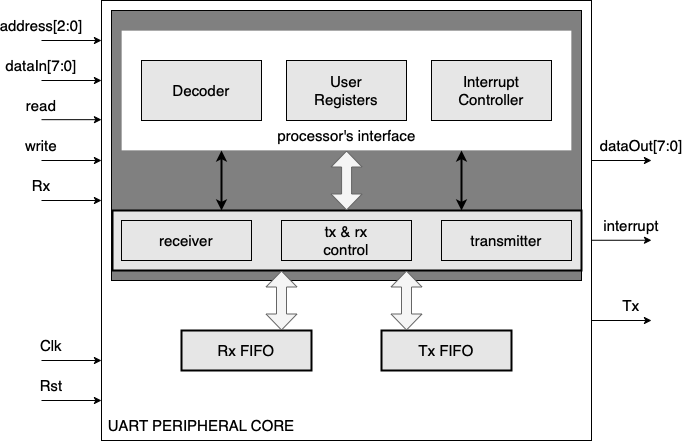
\includegraphics[scale=0.6]{./images/UART}
\caption{MC2101 UART Peripheral Core.}
\label{fig:uart} % \ref{fig:uart}
\end{figure}

The UART module designed for MC2101, whose block diagram is shown in Figure \ref{fig:uart}, provides a transmitter-receiver pair, configurable for different speeds, data widths, parity codifications and information status for several error conditions. The implementation provides a subset of the standard UART 16550 specifications \cite{uart16550}, without including some more advanced functionalities for supporting DMA and MODEM communications.
The module is designed as an 8-bit peripheral and so it provides an 8-bit data interface to the processor. This characteristic makes the Bus Interface more lighter than the GPIO's one, because in this case UART's internal data lines are already compatible with the bus infrastructure of the microcontroller. Also the External Interface is lighter because only two external lines, \texttt{rx} and \texttt{x}, are controlled. Similarly to the GPIO, the signals in Figure \ref{fig:uart} are generated by the Bus Interface, except for the \texttt{rx} and \texttt{tx} lines which came from the External Interface, with the difference that, in this case, the user register file is more compact and requires only 3-bit for the addressing. Both receiver and transmitter use a dedicated queue, implemented in hardware as a FIFO memory, used to hold data either received from the \texttt{rx} serial port or to be written to the \texttt{tx} serial port. This buffering feature is particularly useful when the interrupt mechanism is enabled at the receiver side, which can raise interrupts when its queue surpasses a certain fill level, instead of triggering every time a new character is received. The processor can also benefit from this buffering feature by filling the transmitter's FIFO when multiple character must be transmitted, without the need of wasting polling cycles in waiting for the completed transmission of each character sent. With both the FIFO empty, is possible to have 17 characters simultaneously: in the transmitter, 1 being sent and 16 buffered, while in the receiver, 16 ready to be read and 1 being assembled.

As anticipated, parity conditions and error controls are part of the implemented functionalities. The following error conditions can be detected by the receiver:

\begin{itemize}
\item \textbf{Break Interrupt}: Error flag asserted when the \texttt{rx} line remained stuck at 0 for the entire character time. This error is usually generated from an incorrect wiring, e.g., the \texttt{rx} or \texttt{tx} line are mistakenly wired to a ground pin.
\item \textbf{Framing Error}: Asserted when the stop bit was not detected. Usually this type of error is generated when a device is sending data at a different speed with respect to the one used by the receiving device for sampling.
\item \textbf{Parity Error}: Asserted when the parity of the received character is wrong according to the current one configured. This provides a very simple and useful error detection feature.
\item \textbf{Overrun Error}: Produced when a character is assembled but there is no more space inside the receiver's FIFO. The UART peripheral must be able to inform the processor that it will lose data if the FIFO is not read.
\end{itemize}

Regarding the interrupts, the UART module can be configured to assert an interrupt when different conditions are detected, each one with an associated priority.

\begin{table}
\centering
\begin{tabular}{| p{2cm} | p{2cm} | p{7cm} |}
    \hline
    \textbf{Name} & \textbf{Priority} & \textbf{Description} \\ \hline
    Receiver Line Status & Level 1 (max.) &  There is an overrun error, parity error, framing error or break interrupt indication in the received data on the top of receiver's FIFO.  \\ \hline
    Received Data Ready & Level 2 &  The number of characters in the reception FIFO is equal or grater than the programmed trigger level.  \\ \hline
    Reception Timeout & Level 2 &  There is at least one character in the receiver’s FIFO and during a time corresponding to four characters at the selected baud rate no new character has been received and no reading has been executed on the receiver’s FIFO.  \\ \hline
    Transmitter Empty & Level 3 &  The transmitter's FIFO is empty.  \\ \hline
    \hline
\end{tabular}
\caption{UART Interrupt Sources.}
\label{tab:uartint} % \ref{tab:uartint}
\end{table}

The Table \ref{tab:uartint} summarises the different conditions that can be a source of interrupt and their relative priorities.
\begin{table}
\centering
\begin{tabular}{| p{2cm} | p{2cm} | p{2cm} | p{7cm} |}
    \hline
    \textbf{Name} & \textbf{Address} & \textbf{Access} & \textbf{Description}\\ \hline
    \texttt{IER} & \texttt{0x1A100000} & R/W & Used to individually enable each of the possible interrupt sources. \\ \hline
    \texttt{ISR} & \texttt{0x1A100001} & R & Used to identify the interrupt with the highest priority that is currently pending. \\ \hline
    \texttt{FCR} & \texttt{0x1A100002} & W & Used to reset the FIFOs and program the receiver trigger level for the Received Data Ready interrupt. \\ \hline
    \texttt{LCR} & \texttt{0x1A100003} & R/W & This register controls the way in which transmitted characters are serialized and received characters are assembled and checked. \\ \hline
    \texttt{LSR} & \texttt{0x1A100004} & R & Used to inform the user about the status of the transmitter and the receiver. \\ \hline
    \texttt{DLL} \& \texttt{DLM} & \texttt{0x1A100005} & R/W & Two different registers that together form the 16-bit Divisor Latch, which contains the divisor value used to program the baudrate of the communications. \\ \hline
    \texttt{RHR} & \texttt{0x1A100007} & R & Contains the most recent received character. \\ \hline
    \texttt{THR} & \texttt{0x1A100007} & W & Contains the character to be transmitted. \\ \hline
    \hline
\end{tabular}
\caption{UART User Registers.}
\label{tab:uart} % \ref{tab:uart}
\end{table}
From Table \ref{tab:uart} is possible to see that all registers are on 8-bit and in fact are all byte aligned, with respect to GPIO register file which is word aligned, because all registers are on 32-bit. Another detail is in the RHR and the THR registers, it is possible to see that they are on the same address. This is not a typo. Since RHR is accessed for reading and THR is accessed for writing, it is possible to use the same address for accessing both in an exclusive way. In particular,  during a read operation RHR is accessed, instead, during a write operation the THR is addressed. This trick allows to include all 9 registers in a space that theoretically can only be allocated for 8, saving a bit in the address line.


The UART peripheral can be programmed through the set of registers in Table \ref{tab:uart}. Also in this case, more details about the software are given in the next Section, dedicated to the software part.

\section{Software libraries}
This Section is dedicated to describe the functionalities of the microcontroller from the software point of view. A proper set of libraries is included in the design with the purpose to facilitate the programming of the microcontroller, but also to integrate the possibility to use all the classical string manipulation functions as well as the \texttt{printf} and \texttt{scanf} that are useful also for testing activities.

Before entering into details, the first thing that usually is presented when talking about the programmer's point of view is the memory map of the microcontroller. MC2101 architecture supports a 32-bit address space, which virtually corresponds to a 4 GB memory.

\begin{figure}[h]
\centering
\vspace{0.5cm}
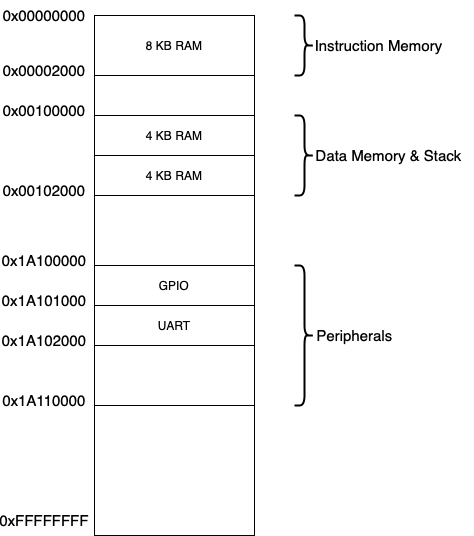
\includegraphics[scale=0.7]{./images/memory}
\caption{MC2101 Memory Map.}
\label{fig:memory} % \ref{fig:memory}
\end{figure}

Figure \ref{fig:memory} shows the default memory map of MC2101. By carefully observing the size of the memory sections it is possible to note that the physical portion of memory currently mapped is in the order of KB, there is a huge free space that can be used in future expansions. In particular the main memory has a lot of available space for being extended to support more advanced software implementations, e.g., hosting an operating system.

The following Subsections are presenting all the possible high-level functions that a programmer can use to write programs for MC2101, maintaining a certain degree of abstraction from the hardware. For this purpose, the GPIO and UART peripherals libraries include a wide amount of functions that, together with macro definitions, allow to program all the functionalities without the need of manually access the user registers manually.

\subsection{GPIO Library}
\begin{table}
\centering
\begin{tabular}{| l | p{7cm} |}
    \hline
    \textbf{Function} & \textbf{Description}\\ \hline
    \texttt{set\_pin\_direction()} & Used to set a pin direction to input or output. \\ \hline
    \texttt{get\_pin\_direction()} & Returns the direction of a given pin. \\ \hline
    \texttt{set\_pin\_value()} & Used to set a pin voltage level to low/high.  \\ \hline
    \texttt{get\_pin\_value()} & Returns a given pin's voltage level.   \\ \hline
    \texttt{set\_pin\_irq\_enable()} & Enable or disable interrupt on a pin.  \\ \hline
    \texttt{get\_pin\_irq\_enable()} & Get the programmed pin's interrupt enable flag.  \\ \hline
    \texttt{set\_pin\_irq\_type()}  & Used to configure the interrupt triggering behavior for a given pin. \{Logic Levels or Edges\}. Pin must have its interrupt flag enabled. \\ \hline
    \texttt{get\_pin\_irq\_type()} & Returns the programmed pin's interrupt triggering behavior.  \\ \hline
    \texttt{get\_gpio\_irq\_status()} & Returns GPIO's current interrupt status register (\texttt{INTSTATUS)} value. Responsible also to deassert the GPIO pending interrupt.  \\ \hline
    \texttt{ISR\_GPIO()} & GPIO interrupt handler. When the interrupt is raised, the bootloader will jump to this function.  \\ \hline
    \hline
\end{tabular}
\caption{GPIO Library functions.}
\label{tab:gpiofunc} % \ref{tab:gpiofunc}
\end{table}

The Table \ref{tab:gpiofunc} shows a simplified prototype and explanation of the GPIO functions currently implemented in the library. The library implements all the necessary functions to be used for programming the peripheral without the need to directly access its registers, thus providing an adequate level of abstraction. The library offers the possibility to configure the direction of each of the 32 pins, read and write values on them. But also, provide a set of functions to be used to enable interrupts on any pin and write a custom interrupt service routine.

\subsection{UART Library}
\begin{table}
\centering
\begin{tabular}{| p{4cm} | p{7cm} |}
    \hline
    \textbf{Function} & \textbf{Description}\\ \hline
    uart\_set\_cfg() &  Used to program the LCR register for configuring the character width, number of stop bits, parity type and enable, even/odd parity and the baudrate.  \\ \hline
    uart\_get\_cfg() &  Return the current LCR register value.\\ \hline
    uart\_set\_int\_en() &  Configure the IER register to enable the different type of interrupt sources. \\ \hline
    uart\_get\_int\_en() &  Used to get the enabled interrupt sources by reading the IER content.\\ \hline
    uart\_rx\_rst() &  Clear the content of the receiver's FIFO.\\ \hline
    uart\_tx\_rst() &  Clear the content of the transmitter's FIFO.\\ \hline
    uart\_set\_trigger\_lv() & Set the receiver's FIFO trigger level.  \\ \hline
    uart\_get\_lsr() &  Used to read the Line Status Register (LSR). \\ \hline
    uart\_get\_isr() &  Used to read the Interrupt Status Register (ISR). \\ \hline
    uart\_sendchar() & Send a character on the transmitter line. \\ \hline
    uart\_getchar() &   Get the character received. \\ \hline
    uart\_send() &  Used to send a string on the transmitter line.\\ \hline
    ISR\_UART() &  UART interrupt handler. When the interrupt is raised, the bootloader will jump to this function. \\ \hline
    \hline
\end{tabular}
\caption{UART Library functions.}
\label{tab:uartfunc} % \ref{tab:uartfunc}
\end{table}

The UART library offers a bigger set of functions with respect to the GPIO library, functions that are also more complex (in terms of execution time) because also the UART features are more complicated. The library provides the possibility to configure the speed of the communications, the size of the frames transmitted/received as well as all the error detection mechanisms. Provides to the programmer functions able to send single characters or strings, and to customise the interrupt behavior.\\
More details about the library are reported in Table \ref{tab:uartfunc}.

\subsection{String Library}
More advanced I/O functionalities have been implemented in the \emph{string} library. This library is particularly important, because it provides the principal string manipulations functions that together with the UART Library are able to support the \texttt{printf} and \texttt{scanf} functions. The library is the same implemented in PULPino, with the addition of the \texttt{scanf} function and some other utilities. The following functions are part of the system's library:
\texttt{strlen}, \texttt{strcpy}, \texttt{strcmp}, \texttt{puts}, \texttt{putchar}, \texttt{memset}, \texttt{printf} and finally the \texttt{scanf}.

\subsection{Board Library}
This is the ``top-level'' library that should be included in every application developed for MC2101. It contains the \texttt{board\_setup} function, which was prepared right after the pin planning phase. It is used to initialize the microcontroller hardware once synthesized on FPGA and connected with the various user buttons, switches and LEDs present in the board.

Once called, the microcontroller is configured in this way:
\begin{itemize}
\item UART peripheral is programmed with 115200 standard baudrate, no parity, 1 stop bit, 8-bit character width. This is a standard configuration for the \texttt{printf} and \texttt{scanf} functions.
\item GPIO lines interconnected to LEDs are set as output.
\item GPIO lines interconnected to User buttons are set as input.
\item GPIO lines interconnected to Switches are set as input.
\item Al interrupts are disabled.
\end{itemize}
The \texttt{board\_setup} function should be the first called in every application, because brings the microcontroller in the correct configuration, according to the pin assignment used for the synthesis, in order to properly interface the external hardware.

\section{Testing}
The microcontroller has been tested with the combination of RTL testbenches and C programs, aimed together to verify the correctness of the architecture. The original AFTAB simulation environment, similar to PULPino, has been adopted and extended for the test of MC2101.

As anticipated, the software environment integrates the RISC-V toolchain with ModelSim commands using CMake build automation tool. In this way, it is possible to compile custom C applications, HDL design files, and also run RTL simulations on ModelSim.

The test of the architecture has been separated into two distinct phases:
\begin{enumerate}
\item Testing while-developing.
\item Testing post-synthesis on FPGA.
\end{enumerate}  

\subsection{Testing while-developing}
Test activities and design activities happened in parallel during the RTL development of the microcontroller. All the components have been implemented using a structural approach in such a way to have a modular design, easily testable with a bottom-up methodology.

\begin{figure}[h]
\vspace{0.5cm}
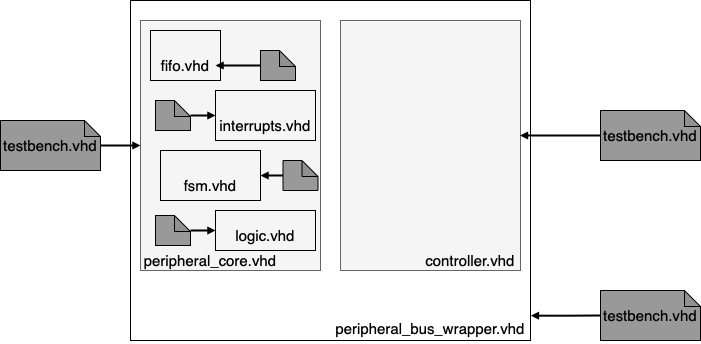
\includegraphics[scale=0.6]{./images/testing}
\caption{Modular structure of a peripheral.}
\label{fig:testing} % \ref{fig:testing}
\end{figure}

Figure \ref{fig:testing} shows what is the typical structure used to design all the peripherals. There is always a top-level entity, that works as a wrapper for the bus controller and the peripheral core, which is itself composed of discrete interconnected HDL entities. Each of the entities is at first tested in isolation, then in integration with the other components until the design is functionally tested from the bottom to the top-level entity. The peripheral can be then attached to the bus, through the top-level wrapper, and be finally tested with a proper C/Assembly program to verify the correctness of the interconnection with the processor and the memory. With this approach, the microcontroller can be testes bottom-up, and debugged with custom applications. After these steps, the final test would be to proceed with the synthesis of the design and perform a last RTL test with a gate-level simulation, to properly check that timing constraints are really respected. 

\subsection{FPGA Tests}
The test procedure explained before is not actually able to fully test all the functionalities because of the limitations of RTL simulations. Interrupts for instance, are ver difficult to test, because they should be generated asynchronously by the external environment, e.g., a button press. Other behaviors like the \texttt{printf} or \texttt{scanf} functions would require very long simulation times (in the order of ms) that can really overload ModelSim, with the risk of crashing the workstation.

In general, the functional properties of the microcontroller can be fully tested only when synthesized on FPGA, that in our case is the Cyclone-V FPGA embedded into the DE1-SoC development board. With the purpose of having a proper test infrastructure, a set of make targets, integrating Quartus commands with tcl and bash scripts have been prepared in order to provide to the user a simple, fast and automatic toolchain for the synthesis and deployment on FPGA. The most useful feature of the aforementioned toolchain, is certainly the possibility of updating the memory content of the sythesized microcontroller with new programs, without having to repeat the entire synthesis process from scratch, which can be quite time consuming.

Below, are presented some more details about the testing of the UART and GPIO peripherals, thus are also showed the different ways of interacting with the microcontroller.

\begin{figure}[h]
\centering
\vspace{0.5cm}
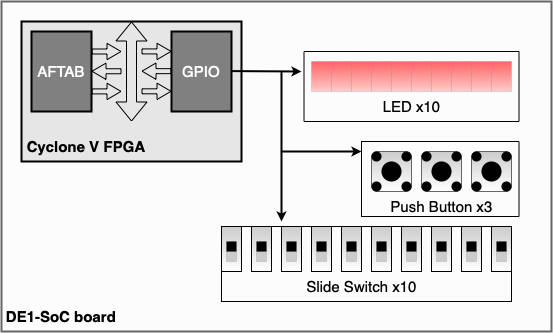
\includegraphics[scale=0.6]{./images/gpiotesting}
\caption{GPIO Interconnection on DE1-SoC.}
\label{fig:gpiotesting} % \ref{fig:gpiotesting}
\end{figure}

\textbf{The GPIO peripheral} is interconnected with a proper set of component present on the DE1-SoC. As shown in Figure \ref{fig:gpiotesting}, there are 10 LEDs in total, 3 push buttons, and 10 switches that are physically connected with the GPIO's External Interface lines. This set of electronic components are very useful in order to test the behavior of the peripheral, the user can assess if the peripheral works or not by just trying to turn on/off LEDs. Test programs have been implemented with the purpose to check the functional correctness of the the whole peripheral and the interrupt mechanism.

\textbf{The UART peripheral} has been tested together with the \texttt{printf} and \texttt{scanf} functions. In this case, the test is a little bit more complicated, as it requires the usage of a Terminal Emulator in order to see if the I/O functions are working. 

\begin{figure}[h]
\vspace{0.5cm}
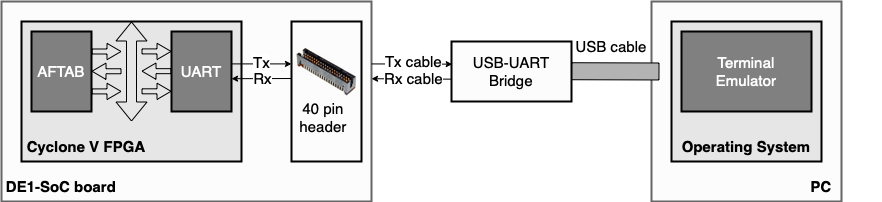
\includegraphics[scale=0.5]{./images/uarttesting}
\caption{UART Interconnections.}
\label{fig:uarttesting} % \ref{fig:uarttesting}
\end{figure}

In Figure \ref{fig:uarttesting}, the communication mechanism designed for interconnecting the UART peripheral with an external PC is shown. The interconnection is very simple, the \texttt{tx} and \texttt{rx} lines have been routed with 2 header pins of the DE1-SoC, then two cables are used to connect the \texttt{tx} and \texttt{rx} lines to a USB-UART bridge that is directly plugged into USB Port of a computer. In this way, every Terminal Emulator is able to print the character transmitted by the microcontroller and also send character to the microcontroller. This communication mechanism, together with the GPIO connections allow a proper test of the entire microcontroller.
\chapter{Experimental Results}
The aim of this Chapter is to show the results obtained from the design choices implemented. In particular, the specifications of the systems are evaluated as well as the FPGA resource usage, which is very useful to know in order to evaluate which future extensions to implement.

Starting from the specifications, as anticipated, the purpose of this project was to design a simple, modular, and extensible microcontroller able to provide all I/O functionalities to support its usage in a realistic environment. All tests performed have shown that the system fulfils all of the requirements. In fact, MC2101 is able to interface correctly with all of the interconnected hardware components of the DE1-SoC. The infrastructure built for bridging the communications between the UART and a Terminal Emulator allows the user to interact correctly with the system by using any platform that have a USB driver inside. Assessed that also the interrupt mechanism fully responds to external triggers, the system requirements have been fully fulfilled.

Thanks to the fact that the main memory has been designed to be synthesised in the embedded M10K blocks of the Cyclone-V FPGA, it is possible to extend the available RAM without wasting LUTs. Considering that only 3\% of the M10K blocks available on the target FPGA are currently used, and that the architecture actually takes advantage of a very small portion of the addressable space there is plenty of room for future developments.

\begin{table}
\centering
\begin{tabular}{| p{3cm} | p{2cm} | p{2cm} | p{2cm} |}
 \hline
 \textbf{Resource Name} & \textbf{Used Amount} & \textbf{Total Amount} & \textbf{Percentage Used}\\ \hline
 \hline\hline
 ALM & 2628 & 32070 & 8\% \\ 
 \hline
 FF & 3443 & 64140  & 5\% \\
 \hline
 PIN & 36 & 457  & 8\% \\
 \hline
 M10K Bit & 131072 & 4065280 & 3\% \\
 \hline
 RAM Block & 16 & 397 & 4\% \\
 \hline
\end{tabular}
\caption{MC2101 resource usage on Cyclone-V FPGA.}
\label{tab:res} % \ref{tab:res}
\end{table}

More details about FPGA resource usage are reported in Table \ref{tab:res}. It is possible to see that the architecture of MC2101 takes advantage of a very small percentage of the available resources on the Cyclone-V, which allows a great deal of freedom for future extensions.

To conclude the discussion, it is useful also to compare the results of the MC2101 synthesis with those of PULPino, which has been the reference architecture and will still be source of inspiration for future developments. Unfortunately, following several attempts, was not possible to correctly synthesize PULPino on the Cyclone-V using Quartus software.

This is due to the outdated release of the software, that does not support some of the SystemVerilog HDL structures coded inside PULPino. For instance, the memories in PULPino are designed to be synthesized within Vivado HLS for Xilix FPGAs that are not supported in Quartus. Because it was not possible to synthesize PULPino using MC2101 synthesis environment, the two architectures have been synthesized using Vivado HLS in order to have a report generated by the same synthesis software and also in order to have a comparison between the architecture that is useful to understand what results to expect from future developments of our microcontroller.

\begin{table}
\centering
\begin{tabular}{| p{3cm} | p{2cm} | p{2cm} | p{2cm} |}
 \hline
 \textbf{Resource Name} & \textbf{PULPino Usage} & \textbf{MC2101 Usage}\\ \hline
 \hline\hline
  LUT & 15657  & 3440\\ 
 \hline
 FF & 9883  & 3253 \\
 \hline
 PINS & 143 & 36 \\
 \hline
 BRAM & 16 & 4 \\
 \hline
\end{tabular}
\caption{PULPino and MC2101 resource usage comparison on Artix-7 FPGA.}
\label{tab:res2} % \ref{tab:res2}
\end{table}

Table \ref{tab:res2} shows the resource usage of both MC2101 and PULPino synthesized on the Artix-7 FPGA using Vivado HLS. As expected, because PULPino implements a typical AMBA-based full-featured design, it is a much more complex embedded system than the current MC2101 and so the resources required for the synthesis are much higher. The memory blocks for instance are 16 instead of 4 because PULPino makes use of 64 KB memory, divided into instruction RAM and data RAM, while MC2101 only uses one 16 KB single port memory. The higher number of peripherals, the pipelined architecture of the processor and the higher complexity of the bus infrastructure are the reasons of which PULPino needs more sequential elements (FF) as well as LUT to implement all the logic required.
\chapter{Conclusions and Future Work}
The goal of this thesis was to provide my research team a RISC-V microcontroller written in VHDL that can be synthesized and usable on FPGA, where is possible to test, integrate and evaluate hardware and software security solutions for embedded systems. The work carried out includes all the functions necessary to automate the synthesis processes, the RTL simulations, the compilation of custom applications and a soft architecture able to run software on FPGA. The architecture designed integrates all the necessary hardware modules e their software libraries required to support all the basic I/O functionalities that permit its usage on a development board. All tests performed have demonstrated the ability of the system to perform all the functions set up, and therefore to be able to satisfy the initial requirements.

The actual state of the platform offers a good starting point for future improvements. In particular, the following are some of the most relevant features that should be included in future extensions in order to have a more complete microcontroller able to run general purpose software:

\begin{itemize}
\item \textbf{Pipelining}: Up to now, all the operations are executed and issued in sequence, thus no pipelined behavior is supported yet and so the performances are the main limitation of this device. Introducing the pipeline into core together with a proper upgrade of the bus infrastructure is indeed a precious feature to be included. This upgrade will definitely increase the computing capability of the embedded system and therefore the possibility to run a wider range of applications.

\item \textbf{ISA Extensions}: In order to support a wider range of applications, the ISA itself must be extended. In particular, for being able to support general purpose computing all the standard extensions \emph{M, A, F, D, C} should be included. Considering that \emph{I} and \emph{M} are already part of the ISA, withe the remaining three standard extensions \emph{F, D, C} the processor will be able to execute floating point single precision (\emph{F}) and double precision (\emph{D}) and also the compressed instructions (\emph{C}).\\

\item \textbf{OS Support}: Currently AFTAB is not able to support the \emph{Supervisor} mode required to run an operating system. Thus, in order to be able to support the full software stack separation required to run an operating system, the ISA must include also the \emph{S} privileged mode and all the required CSR registers. This upgrade, together with the introduction of all the ISA Standard Extensions, would allow the system to run a wide range of general purpose applications.  
\item \textbf{Timer peripheral}: To extend the platform functionalities, there are a lot of peripherals that could be added. For instance, as in PULPino microcontroller, some of the peripherals missing in MC2101 are the SPI, I2C modules and the Timer. What i would suggest more is for sure the Timer peripheral, which is used to trigger periodic interrupts with a very high timing precision. A periodic interrupt can be used for example by the operating system to control the scheduling of processes with a very high timing precision, mandatory feature when real-time constrains must be met. Another example of period interrupt usage is for example the Watchdog Timer, used to generate a non-maskable interrupt that resets the entire system if not handled. This feature is a must, because allows to recover after some bad internal failure occurs and no user intervention is possible. 
\item \textbf{Debug Interface}: All modern MCUs feature an on-chip debug module that opens up the access to all the addressable space, including CPU registers. This capability allows to debug the code execution, that actually in MC2101 can only be performed by dumping contents with the printf function.
\end{itemize}

To conclude, I can say I am satisfied about this thesis experience that allowed me to design the architecture of a system where it is possible to execute real software. I had the opportunity to deepen my skills into the low level design of embedded systems and complete my knowledge on microcontrollers architecture, for which i have grown a great deal of interest during my studies and which i have been able to deepen thanks to this experience. In this regard, I would like to underline the importance of the RISC-V ISA in the world of research and academia and in general the importance of having open-source materials on which is possible to learn, get inspired and create original contribute for the community. As the last thing, I would like to express my gratitude to Gianluca, who constantly supported me during my work, and to Professor Prinetto, who gave me this opportunity.


%
%%%%%%%%%%%%%%%%%%%%%%%%%%%%%%%%%%%%%%%%%%%%%%%%%%%%%%
%    
% HERE IS WHERE YOU INCLUDE YOUR APPENDICES (IF ANY)
%
\appendix
%\input{appendices/appendix.tex}
% and so on
%
%%%%%%%%%%%%%%%%%%%%%%%%%%%%%%%%%%%%%%%%%%%%%%%%%%%%%%

\cleardoublepage
\phantomsection
\addcontentsline{toc}{chapter}{Bibliography}
\printbibliography

\end{document}